\documentclass[letterpaper,12pt]{book}
\usepackage[titletoc]{appendix}
\usepackage[margin=.75in,heightrounded]{geometry}
\usepackage{fancyhdr}

\usepackage[T1]{fontenc}
\usepackage[utf8]{inputenc}
%\usepackage{lmodern}					%font
\usepackage{fourier}                    %font

\usepackage{tabularx}
\usepackage{graphicx}
\usepackage{tikz}
\usepackage{awesomebox}
\usepackage[framemethod=TikZ]{mdframed}
\usepackage{menukeys}
\usepackage{float}
\usepackage{listings}
\usepackage{enumitem}
\usepackage{needspace}
\usepackage{xcolor}
\usepackage{textcomp}
\usepackage{tocloft}
%\usepackage{fontawesome}
\usepackage[singlelinecheck=false]{caption}
\usepackage[hidelinks, linktocpage=true]{hyperref}

\pagestyle{fancy}

\floatstyle{plaintop}
\restylefloat{table}                    % control table placement

\hyphenation{JGNASH}                    % prevent hyphenation
\hyphenation{jGnash}

\parindent0pt  \parskip10pt            % make block paragraphs

\setlength\headheight{16pt}
\setlist[description]{style=nextline}    % newline for descriptive lists

\setlength{\aweboxrulewidth}{0.8pt}    % reduce width the awesome box vertical line
\setlength{\aweboxcontentwidth}{1.0\linewidth}

\renewcommand{\arraystretch}{1.5}        % row height of tables

\renewmenumacro{\directory}[>]{pathswithfolder}     % change icon

\renewcommand\labelitemi{$\bullet$}
\renewcommand\labelitemii{$\circ$}
\renewcommand\labelitemiii{$\bullet$}

\hypersetup{
colorlinks,
linkcolor={blue!80!black},
citecolor={blue!80!black},
urlcolor={blue!80!black}
}

\definecolor{light-gray}{gray}{0.98}    % define light gray backgrounds

\mdfdefinestyle{info}{                    % gray boxes
linecolor=gray,
outerlinewidth=0.25pt,
roundcorner=0pt,
innertopmargin=\baselineskip,
innerbottommargin=\baselineskip,
innerrightmargin=10pt,
innerleftmargin=10pt,
backgroundcolor=light-gray
}

\lstset{%    
backgroundcolor=\color{light-gray},
frame=single,
framesep=1em,
aboveskip=0pt,
stringstyle=\ttfamily,
showstringspaces = false,
basicstyle=\scriptsize\ttfamily,
commentstyle=\color{gray},
keywordstyle=\bfseries,
ndkeywordstyle=\bfseries,
identifierstyle=\ttfamily,
numbers=left,
numbersep=14pt,
numberstyle=\tiny,
numberfirstline = false,
breaklines=true,
columns=fixed,
keepspaces=true,
frameround=ffff
}

\lstdefinelanguage{JavaScript}{
keywords={typeof, new, true, false, catch, function, return, null, catch, switch, var, const, let, async, await, if, in, while, do, else, case, break, from},
ndkeywords={class, export, boolean, throw, implements, import, this},
sensitive=false,
comment=[l]{//},
morecomment=[s]{/*}{*/},
morestring=[b]',
morestring=[b]"
}

\pagenumbering{roman}

\title{\textbf{jGnash 3.2.x Manual} }
\author{Craig Cavanaugh}
\date{\today}

\begin{document}

    \begin{titlepage}

        \raggedleft % Right align the title page

        {\color{gray} \rule{4pt}{\textheight}} % Vertical line
        \hspace{0.08\textwidth} % White space between the vertical line and title page text
        \parbox[b]{0.75\textwidth}{ % Paragraph box for holding the title page text, adjust the width to move the title page left or right on the page

        {\Huge\bfseries jGnash 3.2.x Manual}\\[2\baselineskip] % Title
        {\Large\textsc{craig cavanaugh}}

        \vspace{0.5\textheight} % White space between the title block and the publisher

        {\noindent \today}\\[\baselineskip] % Publish date
        }

    \end{titlepage}

    \tableofcontents
    
    %%%%%%%%%%%%%%%%%%%%%%%%%%%%%%%%%%%%%%%%%%%%%%%%%%%%%%%%%%%%%%%%%%%%%%%%%%%%%%%%%
    \chapter{Legal}\label{ch:legal}
    {\bfseries jGnash Manual}

    Copyright~\copyright~2001-2019 Craig Cavanaugh

    jGnash comes with \textbf{ABSOLUTELY NO WARRANTY}.

    This program is free software: you can redistribute it and/or modify it under the terms of the GNU General Public
    License as published by the Free Software Foundation, either version 3 of the License, or (at your option) any later version.

    This program is distributed in the hope that it will be useful, but WITHOUT ANY WARRANTY; without even the implied
    warranty of MERCHANTABILITY or FITNESS FOR A PARTICULAR PURPOSE. See the GNU General Public License for more details.

    You should have received a copy of the GNU General Public License along with this program.
    If not, see \href{http://www.gnu.org/licenses/}{http://www.gnu.org/licenses/}

    Permission is granted to copy, distribute and/or modify this document under the terms of the GNU Free Documentation
    License, Version 1.3 or any later version published by the Free Software Foundation; with no Invariant Sections,
    no Front-Cover Texts and no Back-Cover Texts.

    A copy of the license is included in the section entitled ''GNU Free Documentation License''.

    Linux\textregistered~ is the registered trademark of Linus Torvalds in the U.S.\ and other countries.
    Windows is a registered trademark of Microsoft Corporation in the United States and other countries.
    Java\texttrademark~ and OpenJDK\texttrademark~ are registered trademarks of Oracle and/or its affiliates.
    
    
    %%%%%%%%%%%%%%%%%%%%%%%%%%%%%%%%%%%%%%%%%%%%%%%%%%%%%%%%%%%%%%%%%%%%%%%%%%%%%%%%%
    \chapter{Conventions and Typographical Features}\label{ch:conventions-and-typographical-features}
    
    Below are conventions used throughout this manual. With jGnash being a cross platform application, there
    may be slight variations in the user interface behavior depending on your operating system. 
    
    \begin{tabularx}{\linewidth}{|l|X|}
        \hline 
        \textbf{Convention} & \textbf{Usage} \\ 
        \hline 
        \hline 
        \keys{CTRL + C} & User Interface buttons, Keyboard shortcuts and individual keys. The \keys{CTRL} key is used generically for \keys{CTRL} and \keys{\cmd} 
        depending on your operating system. \\ 
        \hline 
        \menu{File > Open} & Menu commands with the separator representing a level within the menu hierarchy.\\
        \hline 
        \directory{directory} & Indicates a directory within your operating system. \\        
        \hline
        \hyperref[ch:conventions-and-typographical-features]{Link} & An internal or external hyperlink. \\
        \hline
        \texttt{Monospace} & Example text	\\
        \hline               
    \end{tabularx}      
    
    \mainmatter
    \pagenumbering{arabic}

    %%%%%%%%%%%%%%%%%%%%%%%%%%%%%%%%%%%%%%%%%%%%%%%%%%%%%%%%%%%%%%%%%%%%%%%%%%%%%%%%%
    \chapter{Introduction}\label{ch:introduction}
    
\includegraphics[scale=.6]{images/jgnash-logo-small}

    jGnash is an open source application for personal finances.

    jGnash enables you to record detailed account and transaction information using proven double entry accounting principles.

    You do not have to be an accountant to understand or use jGnash, but jGnash provides options to make new and
    experienced users feel comfortable using it.

    jGnash's mission is personal fiance and it is not tailored for use as a business accounting application.
    jGnash is being used by small businesses and clubs, but if you require business specific features, you may be
    better served looking for a different solution.

    \section{Features}\label{sec:features}
    A brief list of features is below:

    \begin{itemize}
        \item Double Entry Accounting with reconciliation tools.
        \item Budgeting with multiple scenario options and export to spreadsheet capability.
        \item Investment Accounts and automatic import of Stocks, Bond, and Funds price history.
        \item Hierarchical accounts with automatic roll-up of totals and intelligent handling of mixed currencies.
        \item OFX, QFX, mt940, and QIF import with the ability to pre-process using JavaScript.
        \item Reminders and automatic transaction entry and notifications.
        \item Intelligent handling of multiple currencies and exchange rates with automatic online exchange rate updates.
        \item Printable reports with PDF and spreadsheet export capability.
        \item XML, Binary and SQL database file formats.
        \item Operates on most all modern PC operating system \textit{(Java\texttrademark~11 is required)}.
        \item jGnash will utilize multi-core processors.
    \end{itemize}
    
    %%%%%%%%%%%%%%%%%%%%%%%%%%%%%%%%%%%%%%%%%%%%%%%%%%%%%%%%%%%%%%%%%%%%%%%%%%%%%%%%%
    \section{Installation}\label{sec:installation}
    jGnash is not currently distributed with an automatic installation tool.
    You will be required to perform a couple of manual operations that are easily performed for those with a basic
    understanding of how to use a zip file.
    Also, Java\texttrademark~11 or newer must be installed on your computer.

    \textit{\textbf{Use of an OpenJDK package is recommended over use of Oracle JDK due to licensing requirements}}

    OpenJDK is a free and open-source implementation of the Java Platform that is downloadable from various sources.
    Java installation is a simple matter of downloading the correct version for your operating system and using the
    automated installer.

    \begin{description}
        \item[\href{https://www.azul.com/downloads/zulu/}{Azul OpenJDK 11}]
        A branded release that will be easiest to install for most users and is free to use. \\
        \texttt{[https://www.azul.com/downloads/zulu/]}
        \item[\href{https://adoptopenjdk.net/index.html?variant=openjdk11&jvmVariant=hotspot}{AdoptOpenJDK}]
        Will require manual installation but allows more flexibility and is free to use. \\
        \texttt{[https://adoptopenjdk.net/index.html?variant=openjdk11\&jvmVariant=hotspot]}
        \item [\href{https://jdk.java.net/11/}{OpenJDK}]
        Will require manual installation and is free to use. \\
        \texttt{[https://jdk.java.net/11]}
        \item[\href{https://www.oracle.com/technetwork/java/javase/downloads/index.html}{Oracle Java SE 11}]
        Will require manual installation and licensing is required. \\
        \texttt{[https://www.oracle.com/technetwork/java/javase/downloads/index.html]}
    \end{description}

    \notebox{
    If performing a manual installation of Java, The \texttt{JAVA\_HOME} Environment Variable must be set and the
    Java \directory{bin} directory must be in the execution path.
    \newpage
    \bigskip
    If you have multiple versions of Java installed on your computer, The \texttt{JAVA\_HOME} Environment
    Variable must point to Java 11 or newer and the related Java \directory{bin} directory must be the only version
    in the execution path.
    Mixing JVM and JDK versions will confuse the boot loader.
    }

    After Java is installed, you are ready to install jGnash.
    Simply open the zip file and extract the \directory{jGnash} directory and it's complete contents to a directory of
    your choice, and do not alter the files or locations.
    I usually create a directory named \directory{bin} in my home directory and keep
    the \directory{jGnash} directory in it to better organize my computer.
    When upgrading between versions of jGnash, do not unzip to the same location and overwrite the existing files.
    Use a new location or delete the existing files first.

    %%%%%%%%%%%%%%%%%%%%%%%%%%%%%%%%%%%%%%%%%%%%%%%%%%%%%%%%%%%%%%%%%%%%%%%%%%%%%%%%%
    \section{Starting jGnash}\label{sec:starting-jgnash}

    After the \texttt{jGnash} directory has been extracted from the zip file, you should see several files in the directory.
    Of interest at this point are the Bash script and \texttt{exe} files.

    If you are running on a Windows\texttrademark~ based computer, you can simply double click on the \texttt{jGnash.exe} file to
    start jGnash.

    If you are running on a Un*x or BSD (macOS) based system you can start jGnash from a terminal as shown below using
    the included Bash script.
    You can also create your own application launcher using the Bash script in your desktop environment of choice.

    \begin{mdframed}[style=info]
        \texttt{./jGnash}
    \end{mdframed}

    jGnash has several advanced features such as running as a portable application or using jGnash as a multi-user home
    networked application. These advanced features are accessible via the command line.
    Please see \hyperref[ch:cmdOptions]{Command Line Options} for more details.

    \section{Running for the First Time}\label{sec:running-for-the-first-time}
    A license acceptance screen will be displayed the first time you start jGnash.
    jGnash will not run unless the license is accepted.
    The short of the license agreement is jGnash is a freely available program comprised of other freely available software,
    and should anything bad happen during use, the authors are not libel for any damages.
    The license also details how jGnash may be distributed and used.

    \notebox{
    If the license agreement sounds daunting, take a look at the license agreements of commercially available personal
    finance applications and you will see similar agreements.
    Myself and just about every other person making software available for free or purchase tries their best to ensure the
    software they create works well and as intended.
    Sometimes bugs do creep in and it does not work quite as planned.
    The advantage of free software is you generally have direct access to the authors, and you have a much larger voice in
    helping the application grow and evolve over time.
    }

    \section{Getting Help and Giving Back}\label{sec:getting-help-and-giving-back}
    The intent of this user guide is to get you off to a good start using jGnash.
    Despite my best attempts, there are those who need a little bit of extra help or have a special need or
    circumstance and require the help of others that have already been around the block a few times.

    The best place to start is the jGnash user group hosted at \\
    \href{https://groups.google.com/forum/#!forum/jgnash-user}{jGnash-User} \texttt{[https://groups.google.com/forum/\#!forum/jgnash-user]}.

    The user group contains a well rounded group of individuals who can help answer just about any question.
    As a courtesy to others, I encourage you to search the group prior to asking a question to see if it's already
    been answered.

    If you have found a bug, or have suggestions for improvement, the group page has links to a bug and feature request
    tracker that can be used to log and track your requests.
    The group forum can be used to post a bug or request, but use of the tracker ensures the request is not lost in
    the mix of discussions.

    If you are well versed in use of jGnash and other personal finance applications, you are encouraged to give back a
    little time and contribute your experience to the group and help others.

    The~\nameref{ch:frequently-asked-questions} chapter will help answer a few common questions.
      
    % ======================
    % Getting Started
    % ======================
    \chapter{Getting Started}\label{ch:getting-started}
    The basic elements of jGnash are Accounts, Currencies, Securities, and Transactions.
    Every account is assigned one currency and every transaction is associated with at least one account.
    Investment Accounts and Investment Transactions will be associated with a Security.

    jGnash supports various Account types that can be arranged into a flexible hierarchical structure.
    The Accounts may be arranged by financial institution, by type, or some other structure.
    It's good practice to organize your Income and Expense Accounts into a logic arrangement that allows you to drill
    down into a layer of more detail.

    The balance of an Account will roll up into it's parent Account within the Accounts view as well as in some reports.

    Below is a typical Expense Account arrangement that allows you to differentiate between different type of automotive
    and food related expenses, but roll them up into more macro level expenses.

    \begin{mdframed}[style=info]
        \begin{itemize}
            \item Expense Accounts
            \begin{itemize}
                \item Automobile
                \begin{itemize}
                    \item Fuel
                    \item Insurance
                    \item Service
                \end{itemize}
                \item Food
                \begin{itemize}
                    \item Dining Out
                    \item Groceries
                \end{itemize}
            \end{itemize}
        \end{itemize}
    \end{mdframed}

    The Account structure may be changed and reordered later, but Accounts may not be deleted if they contain transactions.

    Transactions are used to record daily expenditures as well as income from the sale of personal items, investments, or
    paychecks.

    If you are familiar with other personal finance applications, you may notice that jGnash uses income and expense
    \textit{accounts} instead of income and expense \textit{categories}.
    Functionally, there is no difference, other than jGnash allows you see a detailed transaction register of the
    income and expense accounts as easily as you would look at your bank accounts.

    \section{Editing Environment}\label{sec:editing-environment}
    The jGnash editing environment is not much different then in other application with the exception that it provides a
    few shortcuts to speed up entry of transactions.

    jGnash knows and understands just about any known locale and country setting.
    Depending on your settings, the decimal symbol will change accordingly as well as the displayed format of dates.

    Error checking of required form fields is performed real-time.
    As information is entered you will notice buttons such as \keys{Enter} are enabled and disabled based on validity
    of what has been entered.

    \subsection{Date Fields}\label{subsec:dateFields}
    The date field is freely editable and jGnash will make the best attempt at interpreting an invalid entry, but the results
    are indeterminate.
    Clicking on the button to the right of the field will display a calendar dialog where you can select a date as well.

    The field is flexible enough to allow use of multiple keys as the field separators regardless of the current locale.
    This is done to make entry easier on compact keyboards.
    The usable field separator characters are defined in the table below.

    
\includegraphics[scale=.8]{images/date-entry}

    Also, dates can be modified using the keyboard shortcuts defined below.

    \begin{table}[H]
        \begin{tabular}{ll}
            \hline
            \multicolumn{1}{|l|}{\textbf{Keys / Mouse}}                            	& \multicolumn{1}{l|}{\textbf{Function}}            \\ \hline \hline
            \multicolumn{1}{|l|}{\keys{{+}} \keys{\arrowkeyup}, Mouse Scroll Up}   	& \multicolumn{1}{l|}{Increase the date by one day} \\ \hline
            \multicolumn{1}{|l|}{\keys{-} \keys{\arrowkeydown}, Mouse Scroll Down} 	& \multicolumn{1}{l|}{Decrease the date by one day} \\ \hline
            \multicolumn{1}{|l|}{\keys{PgUp}, Mouse Thumb Wheel Up}                	& \multicolumn{1}{l|}{Increase the date by one month} \\ \hline
            \multicolumn{1}{|l|}{\keys{PgDn}, Mouse Thumb Wheel Down}              	& \multicolumn{1}{l|}{Decrease the date by one month} \\ \hline
            \multicolumn{1}{|l|}{\keys{t} \keys{T}}                                	& \multicolumn{1}{l|}{Change to today's date} \\ \hline
            \multicolumn{1}{|l|}{\keys{,} \keys{.} \keys{/} \keys{\textbackslash}} 	& \multicolumn{1}{l|}{Valid field separator for all locales} \\ \hline
        \end{tabular}
        \caption{Date Entry Shortcut Keys}
    \end{table}

    \subsection{Number Fields}\label{subsec:numberFields}

    Numerical entry in jGnash is as easy as typing the desired value into the field.
    Decimal separators are handled according to the configured locale.

    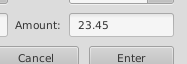
\includegraphics[scale=0.8]{images/basic-decimal-entry} \hspace{10pt} 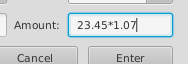
\includegraphics[scale=0.8]{images/advanced-decimal-entry}

    You may also enter arithmetic operators and calculate values within the entry field.

    The arithmetic operators that may be used are \keys{(} \keys{)} \keys{{+}} \keys{{-}} \keys{$\star$} \keys{/} \keys{.} \keys{,}~.

    Traditional arithmetic operator precedence is followed for all calculations.

    \section{Creating a New File}\label{sec:creating-a-new-file}

    When you start jGnash for the first time, you will be presented with a very simple screen.
    At the bottom of the screen application messages and background process indicators are shown.

    \subsubsection*{Creating a new file is done in 5 steps using the wizard}
    \begin{enumerate}
        \item Create a new file using the \menu{File > New} command and follow the prompts in the new file wizard.
        When given the choice to select the \hyperref[subsec:fileTypes]{storage type}, leave it as the default value for now.
        A default file name and location will be provided that you can change if desired.
        If the file already exists, you will be warned you are about to overwrite it.
        \item After selecting the \hyperref[subsec:fileTypes]{storage type} and file name, you will be asked to choose
        the default currency.
        The default currency can be changed at a latter time, and if for some reason your currency of choice is not
        available, you can create a custom currency and set it as the default after the file is created.
        \item Next you can choose the currencies that are available for use.
        Currencies may be added and removed as needed at a later time if needed.

        If needed, custom currencies may be added using the \menu{Currencies > Add/Remove} command.
        As locales change, default currency availability will change as Java is updated.
        The typical need for a custom currency is to support legacy accounting information as countries standardize on the Euro.
        \item After choosing the available currencies, default accounts can be selected if desired.
        If you are new to personal finance software, the defaults will be a good starting point.
        The accounts structure can be easily changed after creating the file to accommodate your own personal needs.
        \item The last step is the Summary page of the wizard.
        Verify everything is to your liking and click on the \keys{Finish} button to create your new file.
    \end{enumerate}

    After the file is created, you are now ready to change, add, or remove accounts as need and begin entering transactions.

    \begin{mdframed}[style=info]
        Encryption and password protection options do not exist in jGnash with the exception of a clear text password
        for client/server operation.

        Encryption is difficult when it involves exporting and distributing software throughout the world.
        jGnash is designed to support many nationalities, so control of distribution would be become very difficult if
        encryption was integrated.

        If you do have the desire to encrypt your jGnash data, the best choice is to use the encryption capabilities
        of your operating system or
        install a freely available third party encryption tool.
    \end{mdframed}

    \subsection{File Types}
    \label{subsec:fileTypes}
    jGnash supports different file types for storing data.
    File types can be easily changed by using the \menu{File > Save As} command and naming the new file with the
    appropriate file extension.

    The current file will be saved in the new format and automatically opened.

    Regardless of file type used, jGnash automatically saves the data if changed every 30 seconds to minimize the
    chance of accidental data loss.

    \notebox{
    If you are using jGnash in the Client/Server mode, all changes are committed immediately.
    }

    \subsection{H2 and HyperSql SQL Databases}\label{subsec:h2-and-hypersql-sql-databases}
    An H2 or HyperSql SQL database is required when using the client / server functionality of jGnash.
    jGnash embeds the database server so that no additional configuration or installation of software is required
    to use a relational database.

    The relational database may be used for a single user.
    If startup and shutdown performance is important to you, then the binary file format described below is a better choice.

    The advantage of the relational database outside the requirement for client / server capability is the ability
    to use several available tools to browse
    and query your jGnash data.
    Also, a relational database is more tolerant of system crashes or power outages vs.\ use of an XML or Binary file.

    The disadvantages of the relational database is a bit slower operation, larger file sizes, and increased memory consumption.

    If using the H2 Database and operating over a network using Client/Server mode, you have the option of enabling
    encryption for network communication.
    This will not encrypt your database file.
    See the Command line options for specifics.

    \notebox{
    The default administrator for a jGnash relational databases is JGNASH and is not configurable at this time.
    }

    \subsection{XML File}\label{subsec:xml-file}
    XML file format is human readable and easily read by other applications at the expense of a considerably larger file size.
    Memory usage is less when using the XML file format, but certain operations may take longer.
    The advantage of the XML file is easier parsing and manipulation of the file using another program external to jGnash.
    If you have a large amount of data, jGnash will use less system memory when using the XML file format.


    \notebox{
    The XML format is also used for creating automatic backups of jGnash files if enabled.
    }

    \subsection{Binary File}\label{subsec:binary-file}
    The binary file format is the most compact file format and will open and close the quickest.
    This is the recommended file format if you do not need client / server functionality and you are using a laptop
    or a workstation with a UPS\@.

    \newpage
    \section{Accounts}\label{sec:accounts}
    Accounts are what you use to organize how you save and spend your money, and where it comes from.
    Account structures can be changed to organize the display of information to suit your specific needs.

    Typically, you will have a separate jGnash account for each savings, checking, investment account, etc.\
    that you have at a financial institution.
    Accounts can be organized under "placeholder" accounts to add different levels of organization.

    For example, if you would like to see a summary of your accounts by financial institution, you can create a placeholder
    account that represents a single financial institution and group your savings and checking accounts from that particular
    institution.

    Maybe you want to see all savings accounts grouped together and checking accounts grouped together.
    It's just a mater of creating placeholder accounts for checking and savings and placing the respective accounts under them.

    The account structure can be easily changed at any time with the exception of removing accounts after they have
    transaction in them.
    Transactions must be manually deleted from an account before you can remove it.

    %\newpage
    \subsection{Creating Accounts}
    \label{subsec:creatingAccounts}
    A new account is created by clicking on the \keys{New} button in the toolbar of the account list view shown below.

    \begin{figure}[h]
        \caption{New Account Button}
        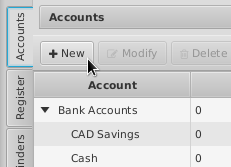
\includegraphics[width=0.4\linewidth]{images/new-account}
    \end{figure}

    A new dialog box will be displayed that allows you to create a new account to suit your particular needs.

    \begin{figure}[H]
        \caption{New Account Dialog}
        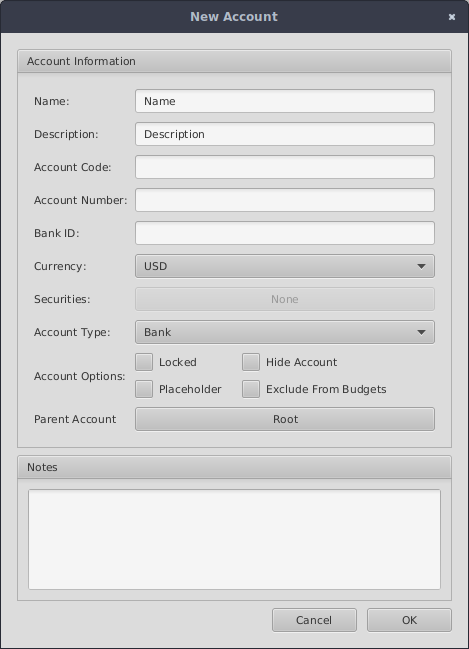
\includegraphics[width=0.55\linewidth]{images/account-dialog}
    \end{figure}

    \subsubsection*{Account Information}
    \begin{description}[style=nextline]
        \item[Name]
        The name for the account.
        The name will be used to identify the account when creating transactions.
        Account names do not have to be unique, but may not be left blank.
        \item[Description]
        A description for the account.
        This field may be left blank if desired.
        \item[Account Number]
        The Account Number field is generally used for storing the account number provided by your financial institution.
        This field may be left blank if desired.
        \item[Account Code (General Ledger Code)]
        The Account Code field will default to a value of 0 and must be a numerical value.
        This value will also control the displayed order of accounts within the same branch.
        If the account code is left as a value of zero, sort order will be deferred to an alphanumeric sort against the account names.
        Best practice is to either use an assigned Account Code for all accounts within the same branch or leave the
        code as a value of 0 for all accounts.
        Otherwise, sort order may appear to be random.
        \item[Bank ID]
        This is the identification number of the financial institution and is generally used as an identifier when importing OFX files.
        This field may be left blank if desired.
        \item[Currency]
        The currency for the account.
        Account currencies cannot be changed if the account contains transactions.
        \item[Securities]
        This button will display a dialog that allows you to add and remove the available Securities for the account.
        This applies only to Investment accounts.
        \item[Account Type]
        Account Type determines what the account can be used for and the type of transactions that can be created.
        An Account's type may be changed after it is created to another type only if it is similar in function.
        For example, an Investment Account can be change to a Mutual Fund account and vice-versa, buy they may not be
        changed into Bank or Credit accounts.
        \item[Account Options:Locked]
        If selected, the account will be locked and further changes will be prevented.
        This is useful to lock accounts that have been closed while retaining your historical data.
        \item[Account Options:Placeholder]
        If selected, child accounts may be placed under this account and the account will not accept transactions.
        This is useful for organizing accounts into a hierarchical structure.
        \item[Account Options:Hide Account]
        If selected, the account is hidden from view if the hide account filter is enabled.
        \item[Account Options:Exclude From Budgets]
        If selected, the account is hidden from view of the budgeting tool.
        \item[Parent Account]
        Clicking on this button will display a dialog that lets you select the account this account resides under.
        If you want the account to be placed at the top most level, then choose the Root account as the parent.
        Parent accounts may be changed as needed to suit your needs.
        \item[Notes]
        Room for extra information about the account if desired.
    \end{description}

    At any later time, the \keys{Modify} button may be used to change an existing account.
    If the account contains transactions, certain options may not be changed.

    \notebox{
    jGnash does not have a place to specify an opening balance in keeping with correct practices for double entry accounting.
    \newpage
    \bigskip
    \textbf{However, it is still possible to set and opening balance:}
    \newpage
    \bigskip
    To add an opening balance, create a transaction with an appropriate deposit or withdrawal against an
    Equity Account of your choice.
    Most people will choose or create an "Opening Balance" account.
    \newpage
    \bigskip
    This follows well known accounting practices.
    \newpage
    \bigskip
    \textit{If you are not concerned about correct accounting practices, you can create an Adjustment Transaction instead.}
    }


    \section{Account Types}
    jGnash allows use of several account types to make organization easier.
    The account type chosen can have a significant impact on how reports are generated and displayed, and the types
    of transactions you can create.

    \subsection{Asset}
    Asset accounts are intended to be used to track the value of durable items such as houses, cars, boats, collections, etc.\
    Value of items can be adjusted over time against Income accounts to show gain or loss of value.
    If you were to sell an item and convert it cash, the sale of the item can be tracked against the Asset accounts containing the item.

    \subsection{Bank}
    Bank accounts are used for the savings accounts you would have at a bank.

    \subsection{Cash}
    Cash accounts represent the cash you carry with you.
    Cash accounts are also good for representing deposits and withdrawals from Flexible Spending Accounts.

    \subsection{Checking}
    Checking accounts are used for the checking account you would have at a bank.

    \subsection{Credit}
    Credit accounts are used to record purchases and payments made to a credit card account.
    Credit accounts are primary used for short-term liabilities and great for representing overdraft and line of
    credit accounts at banks.

    \subsection{Equity}
    Equity accounts are used to record opening account balances against.
    Typically, you will have only one Equity account.
    Equity accounts are representative of another accounts net worth at the time you begin tracking it's value.

    \subsection{Expense}
    Expense accounts are used to record expenses such as food, utilities, taxes, investment expenses, etc.

    \subsection{Income}
    Income accounts are used to record income such as salary, dividends, investment income, etc.

    \subsection{Investment}
    \label{sub:investaccount}
    Investment accounts are used to buy and sell Securities.
    Investment accounts can be used to track 401k, IRA's, etc.
    Please see \hyperref[ch:securities]{Securities} for details specific to setting up Securities.       

    \begin{itemize}
        \item Investment Accounts have a cash balance if you buy or sell transactions against the account.
        \item Investment purchases and sales fees can be made against the cash balance of the investment account or
        other specified accounts.
        \item Multiple investment fee entries per transaction may be entered.
        \item Multiple gains/loss entries per transaction may be entered.
        \item Investment Accounts support multiple securities.
        \item Investment Accounts can be used to model an on-line brokerage account.
    \end{itemize}

    \subsection{Liability}
    Liability accounts are used to track long term loans or liabilities.
    Liability accounts have the added feature of allowing you to set-up a loan payment that takes some of the
    effort out of entering periodic loan payment transactions.

    \subsection{Money Market}
    Money Market accounts are typically a high interest yield account with withdrawal rules or limitations.
    They are generally used for long term savings accounts with the intent of keeping your cash readily accessible.
    Please see \hyperref[ch:securities]{Securities} for details specific to setting up Securities.

    \subsection{Mutual Fund}
    Mutual fund accounts are a specialized version of an Investment account and generally used to track mutual fund type
    investments.
    Please see \hyperref[ch:securities]{Securities} for details specific to setting up Securities.

    \subsection{Simple Investment}
    Simple investment accounts are for investments where you do not actively manage or are able to track purchases and
    sales of securities.
    The typical scenario would be a company pension plan that only provides cash balance information.
    Sometimes, these types of investment accounts are called Annuities or Guaranteed Retirement Accounts

    \subsection{Root}
    The root account is the top level account that holds all other accounts.
    You cannot remove or modify the root account.
    Normally, it is not visible unless you are changing the account structure.

    \section{Entering Transactions}
    jGnash follows well know double entry accounting practices while reducing the complexity of transaction entry.

    If you are familiar with other personal finance applications, you may notice that jGnash uses income
    and expense accounts instead of income and expense categories. Functionally, there is no difference,
    other than jGnash allows you see a detailed transaction register of the income and expense accounts as
    easily as you would look at your bank accounts.

    When creating your file, if you selected the available default accounts, you will have income and expense
    accounts to work with.
    These accounts can be changed to suit your needs at any time.

    The benefit of double entry accounting in jGnash is the ability to use reports and charts to see where your
    money is going and coming from.
    Single entry transactions hide those details and make tracking difficult and tedious.

    \begin{mdframed}[style=info]
        For simplicity, the terms used here to discuss changes in account balances will be \textbf{Increase} and \textbf{Decrease}.

        Business accounting practices use the Credit and Debit terms which can appear to be backwards depending on account type
        and cause confusion for those who are not familiar.
    \end{mdframed}

    \subsection{Common Transaction Properties}
    The properties below are common to all basic transaction types.  \textit{Investment transactions will
    require additional information not covered in this section.}

    \subsubsection*{Payee}
    The Payee is almost always the name of a person or business. The Payee field may be empty, but
    it is good practice to always use a payee for a transaction entry. jGnash will automatically learn
    and auto complete a transaction using the Payee field. This helps aid speed of transaction entry and
    helps to establish consistency making searching and filter much easier.

    \subsubsection*{Number}
    A transaction may be assigned a number or abbreviated description.
    If working with a Checking account, the number is almost always the same as the check number you wrote.
    Use of a check number also makes reconciliation against a bank statement easier.

    \subsubsection*{Date}
    Every transaction has a date that is usually the date the transaction occurred.
    Some people will choose to edit the transaction to match the posting date.

    Please review the \hyperref[subsec:dateFields]{Date Fields} shortcuts that may be used to save a significant
    amount of time when selecting and editing dates.

    \notebox{
    jGnash also maintains an internal timestamp for the actual date and time the transaction was created or last modified
    for auditing and tracking purposes.
    }

    \subsubsection*{Memo}
    The Memo is a brief description of the transaction so you can remember what it was.
    jGnash will automatically learn the Memos you commonly use.
    This helps aid speed of transaction entry and helps to establish consistency making searching and filter much easier.

    Split transactions have an option to Concatenate or automatically merge the Memos of the split entries.

    \subsubsection*{Amount}
    This is the transaction amount. If entering a multi-currency transaction, this field will be expanded to handle
    the correct exchange of currencies.

    The \hyperref[subsec:numberFields]{Number Fields} section details how to enter amounts using mathematical operations
    in the same manner as a calculator.

    \subsubsection*{Reconciliation State}
    The Cleared CheckBox at the bottom of the register form is a tri-state box that allows you to toggle through
    all three of the reconciliation states described below.

    \paragraph*{A jGnash transaction has three reconciliation states}
    \begin{description}[style=nextline]
        \item[Not Reconciled]
        The transaction has not been reconciled against a bank or online statement
        \item[Cleared]
        The intended use is for manual reconciliation of a specific transaction prior to a full reconciliation for the period.
        \item[Reconciled]
        The transaction has been reconciled manually or through use of the Reconciliation tool
    \end{description}

    \subsubsection*{Transaction Attachments}
    jGnash allows the attachment of an image file to the transaction using the chain link button at the bottom of the
    transaction form. The attachment will be moved to a managed directory call \directory{attachments} located in the
    same directory as your jGnash file. The eye button allows you to view the attachment and the broken chain loop
    button allows for removal of the attachment.

    \subsection{Double Entry Transactions}
    A double entry transaction follows standard accounting practices. A double entry transaction will always
    increase the balance of one account and decrease the balance of another account. The amount of the change will
    always equal and opposite in value.

    \begin{mdframed}[style=info]
        Double entry transactions using accounts with different currencies will not be equal and opposite numerically due
        to exchange rates between currencies. jGnash automatically handles the difficult part of the currency exchange
        within the transaction.
    \end{mdframed}

    A double entry transaction normally begins within the register of some type of Cash or Bank account.
    In the example below, a Withdrawal is being made from a Cash account. The balance of the account will be decreased
    by \texttt{25.67} and the balance of the \texttt{Expense Accounts:Automobile:Fuel} will be increased by \texttt{25.67}.

    The account to withdraw funds from (Decrease) or deposit to (Increase) is selected in the Account ComboBox.

    \begin{figure}[H]
        \caption{Double Entry Transaction}
        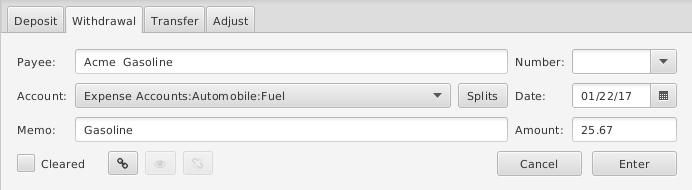
\includegraphics[width=0.9\linewidth]{images/basicDoubleEntry}
    \end{figure}

    \subsection{Split Entry Transaction}
    A Split Entry Transaction is a Double Entry Transaction, but the amount is split across multiple accounts.

    A Split Entry Transaction is started by clicking the \menu{Splits} Button. A dialog will be shown that allows an entry
    for multiple accounts to be made.

    \begin{figure}[H]
        \caption{Split Transaction Entry}
        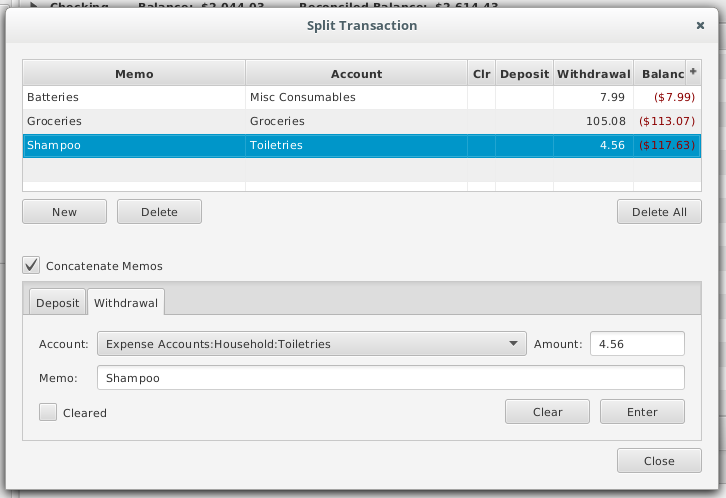
\includegraphics[width=1.0\linewidth]{images/splitTransactionEntry}
    \end{figure}

    Notice the \menu{Concatenate Memos} Checkbox. If the Checkbox is selected, the Transaction memo will be a generated list
    of the unique memos of the split entries. This saves entry time for the Transaction and reduces the file size.

    Editing of the Transaction amount will be disabled as it is the sum of the Entries. The Memo field will be disabled
    as well if the \menu{Concatenate Memos} in the Split Transaction dialog was selected.

    If a memo is not entered for a Split Transaction and the \menu{Concatenate Memos} button is not selected, the
    Transactions register will display the memo of the first Split Entry.

    A Split Transaction may consist of multiple Deposits and Withdrawals as shown in Figure~\ref{fig:mixed-split-trans}. 
    This is a typical example of a paycheck where insurance and taxes are deducted from the gross salary.

    \tipbox{
    Options specfic to reconsiliation of Split transactions will be covered in a later Chapter.
    \newpage
    \medskip
    You have the option of manual reconsiliation, but there are other ways to speed up the process.
    }

    \begin{figure}[H]        
        \caption{Mixed Split Transaction Entry} \label{fig:mixed-split-trans}
        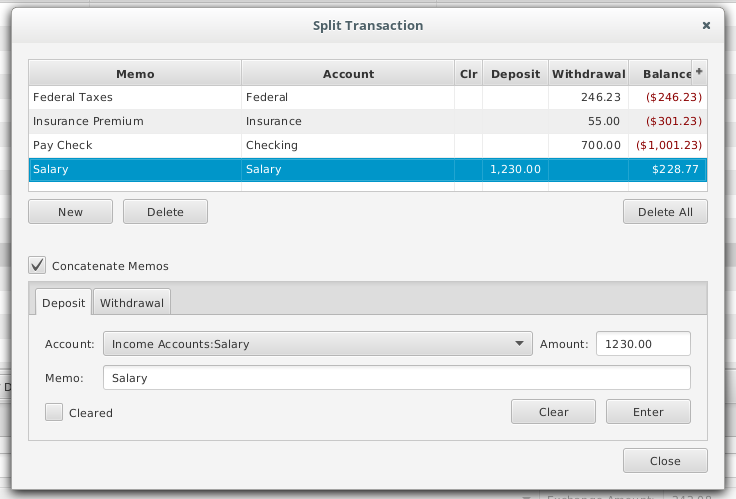
\includegraphics[width=1.0\linewidth]{images/mixedSplitTransaction}               
    \end{figure}

    \subsection{Single Entry / Adjustment Transaction}\label{subsec:single-entry-/-adjustment-transaction}
    A Single Entry Transaction is primarily used to adjust \textit{(fudge)} an Account balance when you simply do not
    have the information to correctly balance the account.

    In Figure~\ref{fig:adjustment-trans}, you can see a negative amount of \texttt{-1.23} was used to decrease the balance of the account.

    \begin{figure}[H]
        \caption{Adjustment Transaction Entry} \label{fig:adjustment-trans}
        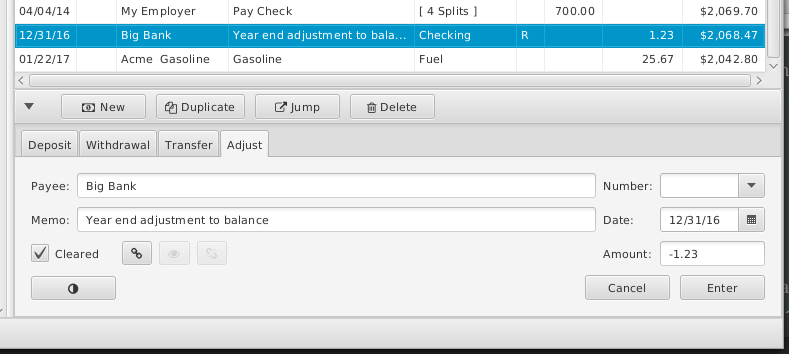
\includegraphics[width=1.0\linewidth]{images/adjustmentTransaction}
    \end{figure}


    The half black and half white circular button at the bottom of the form is a utility to help convert the
    Single Entry transaction into a Double Entry Transaction after you find the needed information.

    \subsection{Transfer Transaction}
    The Transfer tab provides a slightly faster way to move money between accounts without requiring as much information.
    If go back to edit the Transaction, the edits will be performed within the Deposit or Withdrawal forms.
    
    \section{Investment Accounts}
    Investment Accounts need to be populated correctly if the Portfolio report is to work correctly.

    \begin{itemize}
        \item Accounts with prior history should purchase securities from the "Opening Balance" Equity account. Ensure the quantity of
        securities is correct and use the current price.
        \item Cash balances should be transfers from the "Opening Balance" Equity account.
        \item Dividends, sells, etc.\ should occur after opening securities and cash balances are established.
    \end{itemize}

    Please see the \hyperref[ch:securities]{Securities} chapter for details specific to setting up Securities.

    \chapter{Reminders}
    If you find yourself recreating the same transaction on a regular basis, Reminders can be created to automate the process.

    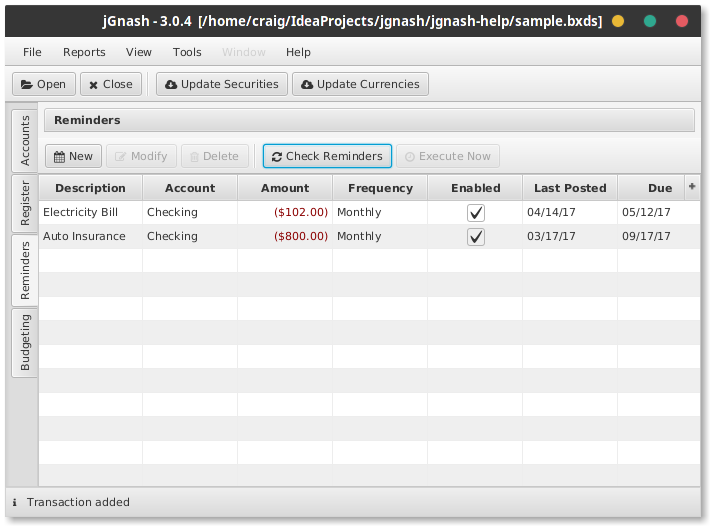
\includegraphics[width=0.8\linewidth]{images/reminders}

    The table shown above displays all the Reminders you have created with some basic information.

    \begin{itemize}
        \item The \textbf{Last Posted} column shows the last date the Reminder was processed. It will be empty for a new Reminder.
        \item The \textbf{Due} column shows the next due date if a configured end date has not been reached.
        \item The \menu{Modify} button is for editing the selected Reminder.
        \item The \menu{Execute Now} button will process the selected Reminder if it is due.
        \item The \menu{Check Reminders} button looks for any pending Reminders and displays them. If there are not
        any pending Reminders, the dialog will not be displayed.
    \end{itemize}

    \section{Notification of Reminders}
    The pending Reminders dialog will be shown shortly after jGnash has been started or when manually checked
    as described earlier.

    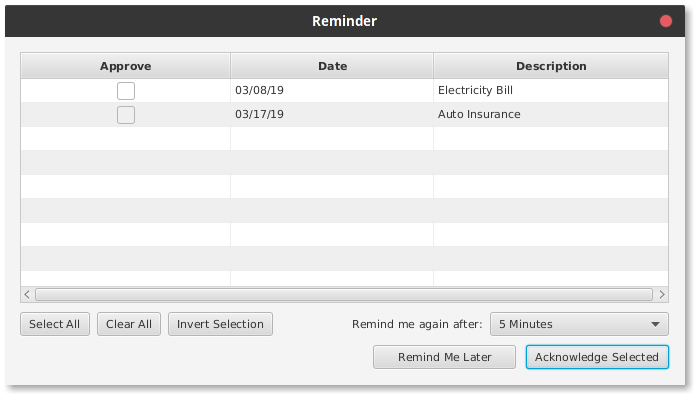
\includegraphics[width=0.8\linewidth]{images/remindersPopupDialog}

    \begin{itemize}
        \item The \menu{Remind Me Later} button lets you to snooze the dialog for a selectable period of time if you do not want to
        process the transactions at that time.
        \item The \menu{Acknowledge Selected} button processes \textit{only} the transactions marked in the \textbf{Approve} column.
    \end{itemize}

    Below the \textbf{Approve} column are buttons to make it easier to mark a large number of transactions for approval.

    \section{Creating New Reminders}

    Creating new Reminders is a process of filling in some basic information, creating your transaction, and configuring the
    frequency of the Reminder.

    An Account must be selected for the Reminder and fields exist to provide a description and additional notes.
    A transaction is optional
    A Reminder without a transaction will simply be a Reminder to do something.

    The typical approach for assigning the Account is to use a bank or cash account of some sort. When you create the
    transaction, it will be against an expense or income account unless it is a periodic transfer between accounts.

    However, if you prefer to organize Reminders by expense type or account, you can pick an expense or income
    account and create the transaction against a bank account.
    Regardless of approach, be consistent to avoid confusion later.

    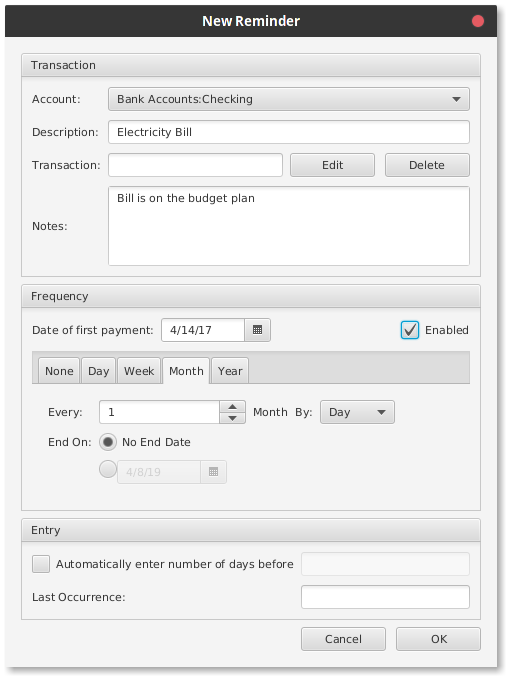
\includegraphics[width=0.8\linewidth]{images/remindersNewDialog}

    Configuring the Frequency of a Reminder is easy despite there being a lot of options. The \textbf{Date of first payment}
    field establishes the first date the Reminder process starts as well as the day of the month it occurs on.

    The \textbf{Enabled} check box will be selected by default. Unselecting it will pause the Reminder should you want
    to disable it for a period of time instead of deleting it.

    The \textbf{Month} frequency tab provides an option of \textbf{Month By Day} or \textbf{Month by Date}.
    As an example, selecting \textbf{Month By Day} indicates you may want a Reminder to occur every 2nd Tuesday of the month.
    Selecting \textbf{Month by Date} would indicate you want a Reminder to occur of the 15th of every month.

    Creating a transaction for a Reminder is identical to creating a transaction in the register. The Date field will be
    ignored and replaced by the recurrence date of the transaction defined in the Frequency section.

    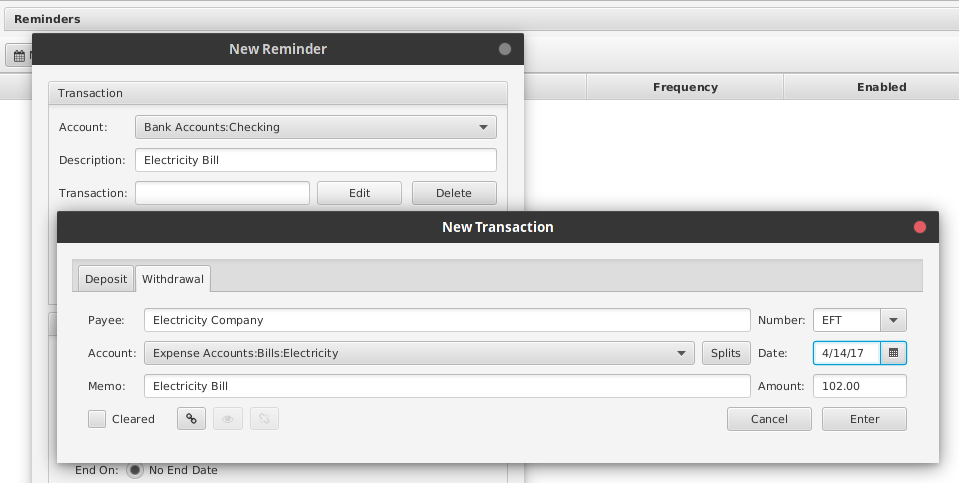
\includegraphics[width=0.85\linewidth]{images/remindersNewTransaction}

    The \textbf{Entry} section of the New Reminder form gives you option to automatically enter a new transaction a defined number
    of days prior to the date defined by the Frequency section. When enabled, you will not see the Notification dialog.
    Typical use is for automatic withdrawals or deposits into an account.

    \section{Tips}

    \subsection{Quick Generation of new Reminders}
    New reminders may be created from an existing transaction.

    Within the Register, right click on a transaction to display the context menu.
    From the context menu, the \menu{Create new reminder} command will generate a new reminder using the existing
    transaction as a template and display the New Reminder Dialog.
    You will need to ensure the Frequency parameters are correct and simply click the\menu{OK} to save it.

    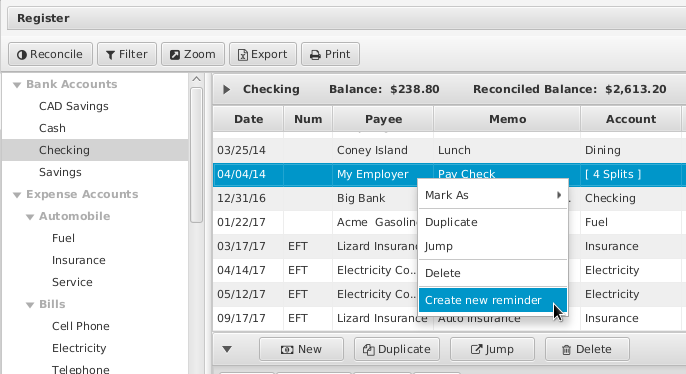
\includegraphics[width=0.8\linewidth]{images/remindersQuickTransaction}

    \subsection{Special Dates}
    Be careful when creating Reminders near the end of the month with a Month frequency.

    \begin{itemize}
        \item What happens if you select February 29th (Leap Day)?
        \item Do you receive a paycheck every two weeks (26 pay periods) or twice a month (24 pay periods)?
    \end{itemize}

    jGnash makes the best attempt to ensure correctness of dates, but minor date shifts can occur should you select leap days,
    the 1st day of a 5 week month, etc.

    \chapter{Budgets}

    jGnash has a budgeting feature that makes it easy for you to define spending and income goals by account and bump those goals up against your actual transactions.
    A compact graphical overview of each budgeting period is provided to highlight how well you are following your budget based on selectable periods.

    Tracking how well you follow your budget can be an eye opening experience and can lead to better financial health.

    \notebox{
    jGnash budget periods follow rules established by ISO 8601. Weeks begin on Monday and the first week of the year may begin
    with the last few days of the prior year.
    }

    \section*{Budget Features}

    \begin{itemize}
        \item Multiple budgets are supported and may be copied making it easy to try out different scenarios and create year specific budgets if desired.
        \item Allowed accounts for budget are limited to Income and Expense accounts.
        \item Accounts may be excluded from budgets by setting the exclude flag in the account properties dialog. Sub-accounts will not be displayed if the parent account is excluded.
        \item The reporting period for budgets may be daily, weekly, bi-weekly, monthly, or quarterly and can be changed as needed.
        \item The per account budget goals may also be entered in daily, weekly, bi-weekly, monthly, or quarterly periods and are independent of the budget reporting period.
        \item The budget may be exported to a spreadsheet.
    \end{itemize}

    \tipbox{
    The reported period of the budget is independent of the per account budget goal period.
    \newpage
    \medskip
    Example: Your salary is paid in bi-weekly intervals, but you want to see your budget reported by month.
    You can change the period for the income account to weekly or daily and enter your salary.
    \newpage
    \medskip
    When reported by month, jGnash automatically handles the difference in the periods and distributes your bi-weekly
    salary income across monthly boundaries.
    }

    \section{Graphical Overview}

    The main budget panel is shown below.

    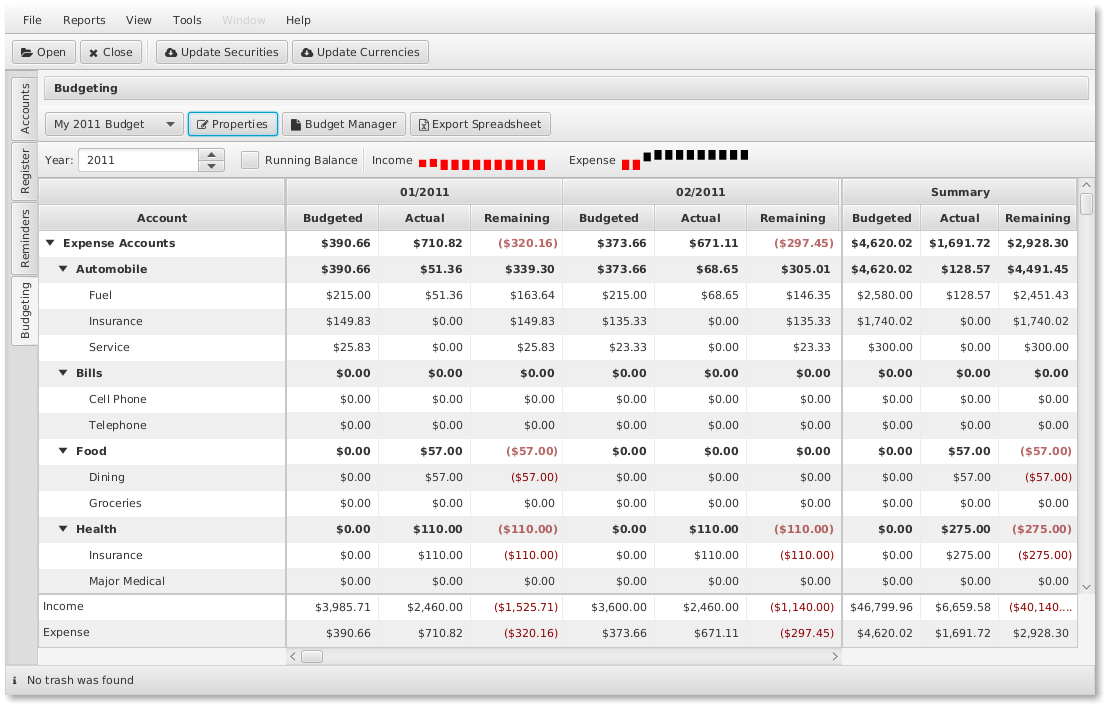
\includegraphics[width=1.0\linewidth]{images/budget-overview}

    The width of the account column is adjustable by placing the cursor between the Account header and the period header
    columns and then clicking and dragging the mouse cursor right or left.

    At the top of the panel, a toolbar exists that allows you to change how much information is displayed, modify the
    budgets, and export the active budget to a spreadsheet.

    The budget drop down list lets you quickly select between different budgets you have created.
    The \menu{Budget Manager} button displays a dialog that let you create, duplicate, and delete budgets.

    The year spinner allows you to bump the selected budget up against the selected year's transaction data.
    The selected year also effects the calendar periods when editing period amounts.

    \subsection{Properties}\label{subsec:properties}
    The \menu{Properties} button will display the dialog shown below with various options for the active budget.

    The period used for the budget display can be changed in this dialog as well as the budget description.
    You may also select the account groups that are visible for the selected budget.

    The \textbf{Start Month} property sets the month you begin a new budget. For most, it's the beginning of the year, but
    others may prefer a month such as April which is tax season for some. If you are new to jGnash and you've started
    mid-year, then the month you being is a good start. The \textbf{Start Month} may be changed at any time without negatively
    impacting your budget goals.

    Regardless of the \textbf{Start Month} selected, jGnash will use a rolling 12 month period based upon the \textbf{Start Month} you
    have selected.

    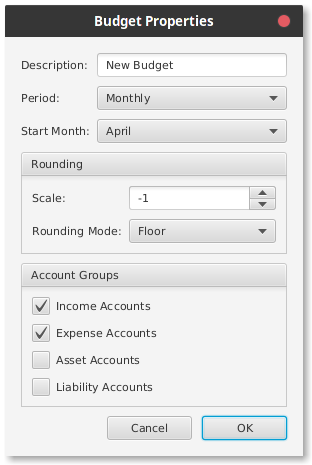
\includegraphics[width=0.5\linewidth]{images/budget-properties}

    The rounding method and number of decimals used to report budget results may be changed.
    The default Rounding Mode is \textit{Floor} which will round up expenses and round down income values which is a conservative
    view of current income and expenses.

    \begin{table}[H]
        \begin{tabular}{|l|l|}
            \hline
            \textbf{Mode} & \textbf{Description} \\
            \hline
            \hline
            Ceiling & Rounds towards positive infinity \textit{(Optimistic View)} \\
            \hline
            Down & Rounds towards zero \\
            \hline
            Half Down & Rounds towards nearest neighbor or down if equal distance \\
            \hline
            Half Even & Rounds towards nearest neighbor or towards even if equal distance \\
            \hline
            Half Up & Rounds towards nearest neighbor or up if equal distance \textit{(Banking)} \\
            \hline
            Floor & Rounds towards negative infinity \textit{(Conservative View)} \\
            \hline
            Up & Rounds away from zero \\
            \hline
        \end{tabular}
        \caption{Rounding Modes}
    \end{table}

    Reported values are rounded based on the selected value for \textbf{Scale}. Negative values for \textbf{Scale} will round to the
    left of the decimal point while positive values round to the right of the decimal point.

    The upper limit of the \textbf{Scale} option is limited by the largest \textbf{Scale} value of the Currencies you have configured.
    \newpage
    \subsection{Budget Management}
    Double clicking on an account name to the left of the panel will display a dialog that allows you to change the account
    specific budget period and period amounts.

    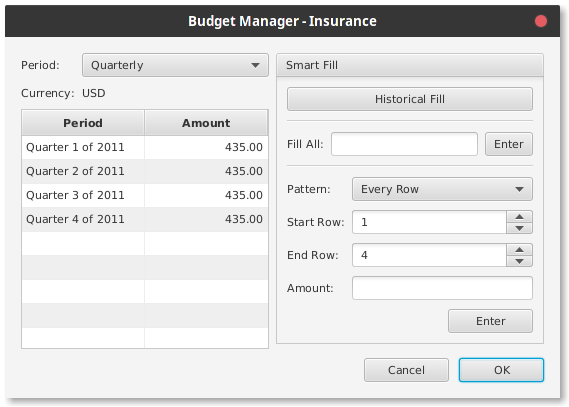
\includegraphics[width=0.8\linewidth]{images/budget-goal-dialog}

    The Smart Fill panel may used to enter repeating patterns or fill in the amounts automatically based on the last 12 months.
    Alternatively, you may directly edit the amount of each period by clicking and typing in a table cell.

    The per account budget amounts as well as the \textbf{Change} and \textbf{Remaining} values are hierarchical in that the values of the child account
    are summed and are added to the parent account. If a parent account is not configured has a placeholder, it may also be assigned
    period goals that are inclusive of any children.

    At the bottom of each reported budget period, a summary by account group is displayed.
    To the right, a summary by account is displayed.
    The summary's made be disabled if desired by unselecting the appropriate check boxes.

    The \menu{Export Spreadsheet} button will export a file to your choice of an \texttt{.xls} or \texttt{.xlsx} file.
    The exported spreadsheet does contain formulas which makes it easier to manipulate the file externally.

    \subsection{Budgeting Tips}

    When planing a budget, you need to consider how you spend and receive your money versus how you want to report your budget.

    jGnash has to make assumptions when entering per account period amounts.
    Internally, jGnash is keeping a list of 366 days (365 + 1 leap day) per account with the list starting at the first
    calendar day of the year.

    When a period goal for an account is entered, the amount is averaged across each day of the period.
    Entry of amounts is also sensitive to the current year.
    If you select Monthly for the account period, the monthly boundary for days is established by the current year calendar
    months and the amount is then averaged across the number of days per each month.

    Averaging of periods has an impact on how exact the tracking of your budget is.
    If you choose to enter a monthly average for income, but are paid on certain days on the month, your budget will show
    slight variations through the year.

    If you want the budgeted vs.\ Remaining amounts to be exact for a particular account, then you will want to set the
    account period to be Daily and take the effort to enter your daily amount goals.

    Minor discrepancies can occur during leap years due to the extra day. Budgets are typically dynamic due to continuous
    changes in income and expenses which means you will naturally address these small discrepancies as you maintain your budget

    You will not be able to export a spreadsheet when the report period is daily due to memory requirements and limitations
    of some spreadsheet applications.

    \chapter{Reconciliation}
    Reconciliation is a simple and visual process of matching up the transactions listed in an account's register against a
    paper or electronic statement provided by a financial institution.
    If differences do exist, then any missing or erroneous transactions must be addressed until the differences are resolved.
    Statements should come from you bank, investment broker, credit card issuer, etc.\ on a periodic basis.

    Periodically reconciling an account helps ensure transaction entry errors do not creep in over time.

    \tipbox{
    Reconciliation is also a great tool for monitoring your accounts for fraudulent transactions.
    }

    Accounts may be reconciled using a manual process or using the Reconciliation Wizard.
    For any given reconciliation period, using a combination of both methods will be difficult.

    Regardless of the Reconciliation process used, it is good practice to reconcile all accounts periodically.

    \section{Basics}
    Every transaction entry will have two independent reconciliation states that applies to both of the related
    crediting and debiting accounts.
    Split transactions may have even more reconciliation states depending on how many accounts it touches.
    Reconciliation states are explained a bit later in this chapter.

    The default assumed reconciliation states can be configured depending on your preferred method of reconciliation.
    Taking time to understand these options is important for a successful reconciliation process.

    \tipbox{
    If this is your first time reconciling an account and you have prior transaction history with a mix of
    Reconciled and Cleared transactions, you may need to manually reconcile prior transaction history.
    }

    \subsection{Reconcile Settings}

    jGnash makes it easier to manage reconciliation by providing some options described below.
    These can be access in the \textbf{Register} options tabs using the \menu{Tools > Options} menu.

    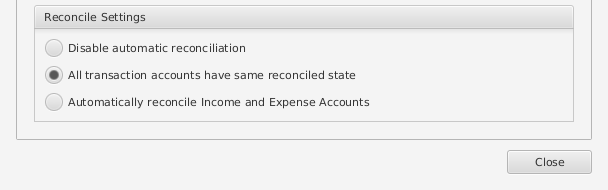
\includegraphics[width=0.8\linewidth]{images/reconcile-options}

    Unless you have very specific needs, it is recommend that you choose to have the option \textbf{All transaction accounts have
    same reconciled state} or \textbf{Automatically reconcile Income and Expense Accounts} selected as the default.

    Selecting \textbf{Automatically reconcile Income and Expense Accounts} requires a bit more work on your part in that you are
    required to reconcile all institution statements, but it will not create any issues when transferring between accounts.
    \textit{This is the recommended option if you are using the Reconciliation Wizard.}

    Selecting \textbf{All transaction accounts have same reconciled state} will reduce the effort of reconciling transactions,
    but can create problems reconciling transfers between bank accounts later. If you manually reconcile your accounts and
    do not use the Reconciliation Wizard, this option saves a significant amount of work at the risk of making an assuming
    a transaction occurred correctly between two institutions.
    \textit{Use of this option in conjunction with use of the Reconciliation Wizard can create problems with bank transfers when
    you reconcile both accounts.}

    Choosing to disable automatic reconciliation will require you to reconcile Income and Expense accounts for which you
    may not have been provided a reconciliation statement.

    \subsection{Reconcile States}

    jGnash transactions have three reconciliation states that are presented in order below:

    \begin{description}[style=nextline]
        \item[Not Reconciled]
        The transaction has not been cleared or reconciled.
        \item[Cleared]
        The transaction has been marked by the user to have been cleared during a manual or unfinished reconciliation process.
        A transaction may be marked as cleared to draw attention to it without impairing use of the reconciliation wizard.
        \item[Reconciled]
        The transaction has been automatically or manually reconciled.
    \end{description}

    \warningbox{
    Manually marking transactions is not recommended if you are going to use the Reconcile Wizard.
    }

    \section{Manual Reconciliation}
    Manual reconciliation is the process of individually comparing the account register against the institution provided
    statement and marking the matching transactions as reconciled.

    The downside to manual reconciliation is not all checks and balances are performed against the reported opening and
    closing balance for a given period. This increases the likely-hood of missing a recorded transaction or incorrectly
    entered amount.

    To manually mark a transaction as reconciled, use the context menu in the register to display options to change the
    reconciled state.

    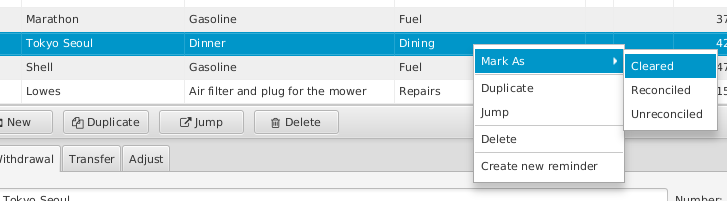
\includegraphics[width=1.0\linewidth]{images/manual-reconcile-context}

    \begin{mdframed}[style=info]
        Use of the context menu is currently the only means of marking a transaction as reconciled other than using the
        reconciliation tool. It may also be used to clear transaction erroneously marked as reconciled.
    \end{mdframed}

    Transactions may also be marked as \textbf{Cleared }through the transaction form.
    Some users may prefer to clear certain transactions manually during a given period to draw attention to them.
    \textbf{Cleared} transactions will still be visible within the Reconciliation Wizard if used later while manually
    \textbf{Reconciled} transactions will not.

    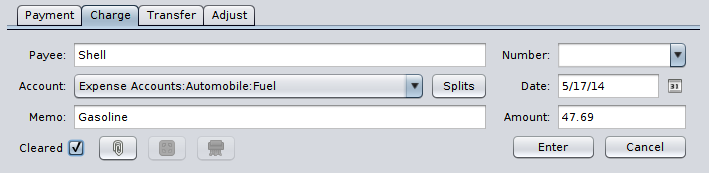
\includegraphics[width=1.0\linewidth]{images/transaction-form}

    \section{Reconciliation Wizard}
    Use of the Reconciliation Wizard helps to simplify the reconciliation process by comparing opening and closing balances
    reported by the institution against the sum of the transactions as you mark them as reconciled. You receive
    instantaneous visual feedback as you mark transactions, and at the end of the process you should have a net difference
    of zero.

    \tipbox{
    The Reconcile Wizard has a nice feature that is not immediately obvious. While the wizard is displayed, you can still
    go back to the account register and enter missing transactions, correct erroneous amounts, or modify and delete
    transactions if entered into the wrong account. The Wizard's credit and debit lists are fully dynamic.
    You are not required to exit the Wizard without completing the process if you discover missing transactions or errors.
    }

    he image of the account register shown next is representative of a small but typical reconciliation period.
    The amounts and balances shown correspond with the other images as the Reconcile Wizard is explained in this chapter.
    Refer back to this image as necessary for clarification.

    Take note of the \texttt{Reconciled Balance:\$2,614.43} and that it is the last transaction marked as reconciled.
    Also, take note of the transaction dated \texttt{03/25/14} and the corresponding balance of \texttt{\$1,369.70}.
    You will see these same values later in the Reconcile Settings dialog.

    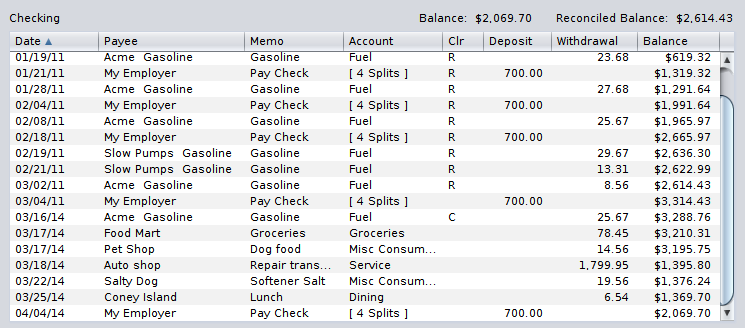
\includegraphics[width=1.0\linewidth]{images/reconcile-register}

    The Reconcile Wizard is started by using the context menu in the Account List, or by clicking the \menu{Reconcile}
    button in the transaction register.

    A small dialog will be shown requesting some information.

    \begin{description}[style=nextline]
        \item[Statement Date]
        This is the closing date for the reconciliation period.
        This should be reported on your account statement.
        The date will typically be the end of the month, but may be different due to institution or locale rules.
        Transactions entered after this date will not appear within the Reconciliation Wizard
        \item[Opening Balance]
        The opening balance should also be provided by your institution and should be equal to the closing balance
        of the last reconciliation period.
        In your account register, this will also be the account balance of the last reconciled transaction.
        \item[Ending Balance]
        This amount should also be provided by you institution.
    \end{description}

    \textit{These values should be provided to you by your banking institution in paper or electronic format and
    it's important these values are entered correctly, otherwise balances will not zero out.}

    Pay special attention to the account type, the selected option for \textit{Reverse Displayed Account Balances}
    and if you are entering a positive or negative opening and ending balance.

    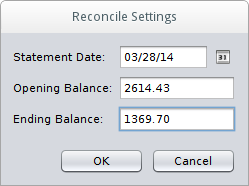
\includegraphics[width=0.4\linewidth]{images/reconcile-settings}

    After clicking the \menu{OK} button, the settings dialog will be replaced by a
    dialog showing all of the transactions prior and inclusive of the statement date
    that have not been marked as Reconciled. \textit{Transactions marked as cleared will be shown.}

    The next step is to go through the institution provided statement and mark every
    matching transaction as reconcilable by clicking on the transactions. As you
    click each transaction, totals will update and you should see the
    \textbf{Difference} value approach zero. The symbol in the \textit{Clr} column will
    also change when marked as \textbf{Reconciled}. When the \textbf{Difference} is zero,
    the \menu{Finish} button will become active. Transactions marked as cleared will
    also need to be selected if they are to be reconciled.

    It is not unusual to find transactions that go unmarked for reconciliation near
    the end of the statement period. These are transactions you have entered that
    were not processed through the system fast enough to show up on your statement
    and impact your account balance. Simply ignore these transactions and they will
    be captured at the start of the next statement and reconciliation cycle.

    \newpage
    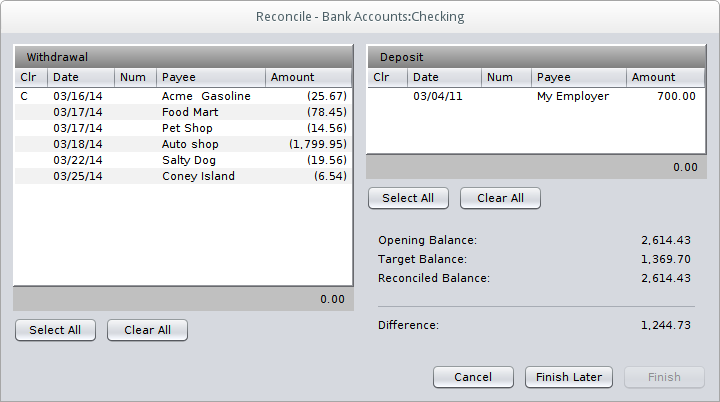
\includegraphics[width=0.8\linewidth]{images/reconcile-dialog}

    Clicking on the \menu{Finish} button will close the dialog and will mark the selected transactions as Reconciled.
    Depending on the number of transactions and type of file format being used, it could take awhile for the changes
    to be saved.
    A wait message will be displayed during the change process.

    What do you do if you have marked all transactions as reconciled and the difference is not zero?

    \begin{itemize}
        \item Not all paper and electronic statements clearly identify fees, earned
        interest, etc.\ Make sure you have captured these transactions.
        \item Were any transactions amounts entered incorrectly?
        \item Transactions manually marked as Reconciled during the statement period will
        not show in the transaction columns and are guaranteed to throw off balances.
        Mark the transactions as \textbf{Cleared} instead.
        \item Do you have your Reconcile Settings configured appropriately for the process
        you are using? If in doubt, use \textbf{Automatically reconcile Income and Expense Accounts}.
        \item Incorrectly entered opening and ending balances will cause errors in calculated balances.
    \end{itemize}

    If you need to to exit the Reconciliation Wizard before finishing, the \menu{Finish Later} button may be used.
    This will close the dialog and mark selected transactions as \textbf{Cleared}.
    This makes it easy to restart the process with transaction you have already marked as reconcilable identified.
    You will still need to re-select those transactions when you restart the process.

    \chapter{Securities}
    \label{ch:securities}
    Securities management is required when entering Investment Transactions within jGnash.  
    
    Securities are typically traded through a financial institution with fluctuating prices and 
    depending, fees may be charged to conduct trades.
        
    At a minimum, a Security is assigned a unique Symbol, a base currency and a Scale \textit{(the number of decimal places 
    for entering and reporting prices)}.  

    Tracking of prices and historical information is optional and not required to enter
    investment transactions.  However, price data will be used for updating the current \textbf{Market Balance} of an account.
    
    
    \section{Create and Modify Securities}
    
    Securities may be created or modified using \menu{Tools > Securities > Create / Modify\ldots}.  All fields are
    accessible when modifying an existing Security.
    
    To create a new Security, fill out the form and click the \keys{Apply} button to save.
    
    You can modify an existing Security by selecting it in the list to the left and click 
    the \keys{Apply} button to save the changes.
    
    \begin{figure}[h]
        \caption{Create / Modify Securities}
        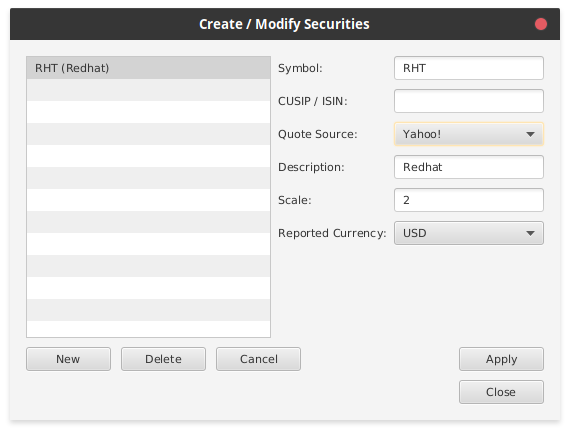
\includegraphics[width=0.6\linewidth]{images/createModifySecurities}
    \end{figure}

    \begin{description}[style=nextline]
        \item[Symbol \textit{(required)}]
        The Symbol is typically the Ticker symbol assigned to the Security.  Depending on the Quote Source used,
        the Symbol my be appended with a market or region code. This value may be left empty.
        \item[CUSIP / ISIN]
        A internationally unique identifier for a Security.  Some Quote Sources may require use of this field
        instead of using the Symbol.  At this time, it is not required. 
        \item[Quote Source \textit{(required)}]
        The Quote Source is the online source chosen to download prices and events.  This is discussed later 
        in the chapter.
        \item[Description]
        A general description for the Security.  This value may be left empty.
        \item[Scale \textit{(required)}]
        This is the number of decimal places used for entry of security prices.  Mutual funds will typically
        be traded at fractional prices.  This allows you to override the number of decimal places used by the
        Reported Currency.
        \item[Reported Currency \textit{(required)}]
        Sometimes called the Base Currency, this is the currency the Security is being traded with.        
    \end{description}        
    
    \subsection{Quote Sources}
       
    jGnash currently supports use of Yahoo and IEX Cloud as online data providers.
    
    \subsubsection{None}
    The default quote source is \textbf{None}.  If used, all pricing, stock splits and dividends will
    need to be entered manually.
    
    \subsubsection{IEX Cloud}
    Using IEX Cloud as a Data Provider requires opening an account which may be free for use or a paid
    subscription depending on the amount of data being consumed. 
    
    An account can be created at \href{https://iexcloud.io/}{IEX Cloud} \texttt{[https://iexcloud.io/]}.
    After creating your account, the \textit{Secret Key} must be entered into the Data Providers Options Tab
    as shown below.  
    
    The \textit{Secret Key} is stored within your jGnash file.  If the key is not entered,
    jGnash will report an error when attempting to download information.
    
    \begin{figure}[h]
        \caption{Data Providers}
        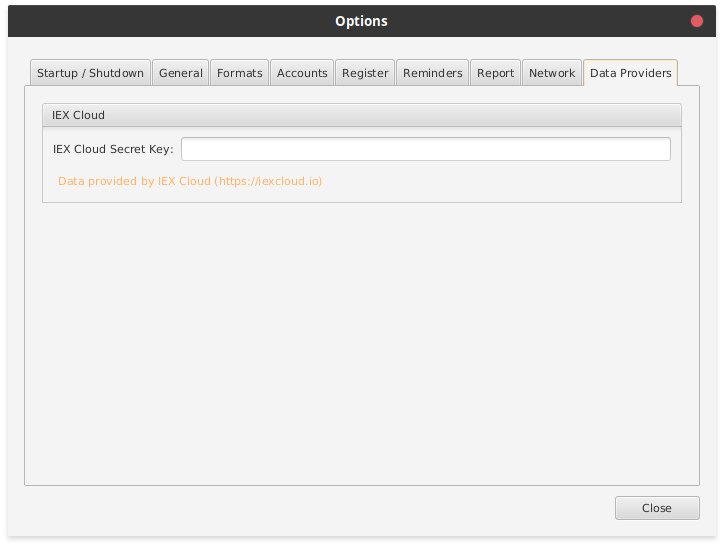
\includegraphics[width=0.6\linewidth]{images/dataProvidersTab}
    \end{figure}
    
    \subsubsection{Yahoo}
    Prices and historical events are downloaded from \href{https://finance.yahoo.com/}{Yahoo Finance} \texttt{[https://finance.yahoo.com/]}.
    Usage is subject to the conditions and terms of the Yahoo website.
    
    Yahoo does not make all Securities available, and it is not uncommon to experience periods of inaccessibility.
    
    \subsection{Security Price History}
    
    Securities history is managed using \menu{Tools > Securities > History\ldots}.
    
    The \textbf{Security} of interest is selected at the top of the form.
    A chart is displayed using on the historical closing price.  
    As shown in Figure \ref{fig:securitieshistorydialog}, periods divided by a stock split 
    are shown using a different color.
    
     \begin{figure}[h]                          
        \caption{Modify Securities History}                  
        \label{fig:securitieshistorydialog}   
        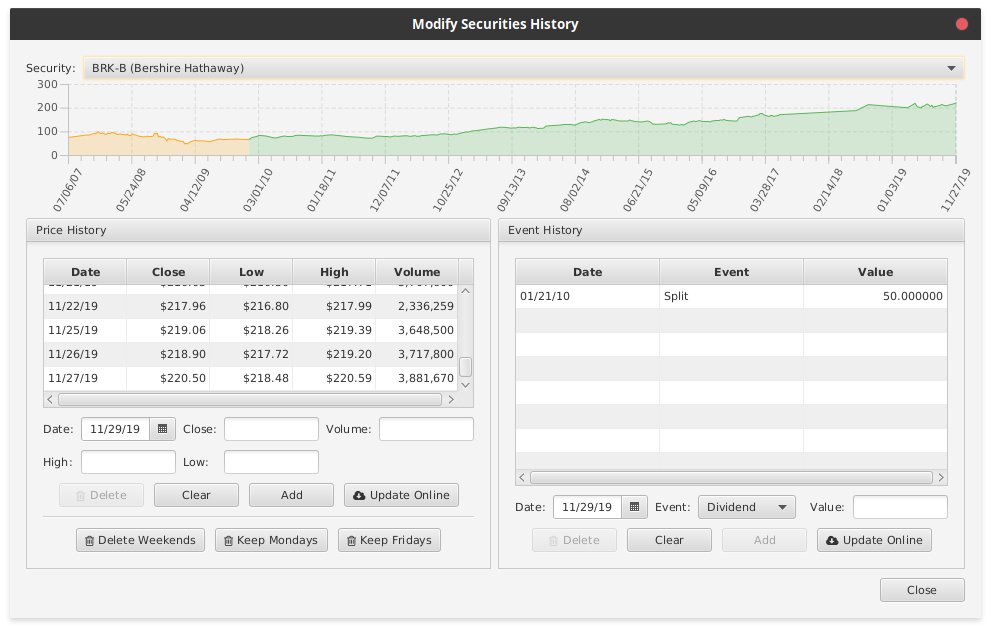
\includegraphics[width=1.0\linewidth]{images/modifySecurityHistory}
    \end{figure}
    
    \subsubsection{Price History Panel}
        
    The closing price as well as the daily high, low and trade volume can be filled in and added by clicking
    on the \keys{Add} button.  The \keys{Clear} button will reset the entry form.  Selecting a date in the list
    and clicking the the \keys{Delete} button will permanently remove the entry.
    
    At the bottom of the \textbf{Price History Panel} are some convenience buttons to help pare down the amount of data
    that can accumulate over time.  
    
    Thinning out the data can significantly reduce the size of your file and improve application performance.
    
    Please see \hyperref[sec:pricelookup]{Price Lookup and Reporting} Section for specifics of how jGnash uses
    the Price History for reporting and estimating Investment Account balances.
    
    \subsubsection{Event History Panel}
    
    Similar to the \textbf{Price History Panel}, Dividends and Splits may be entered.
    
    Dividends can be added for informational purposes but are not required.
    
    Split entries help to correctly manage the visual trend of the chart.  They are not used or required
    to correctly calculate the value of your Investment Account.
    
    \warningbox{
       When Splits or Diviends do occur, it's important
       to remember to create a Split Transaction within the Investment Account register.  
       Splits and Dividend chart events do not automatically register has transaction events.
    }
    
    \tipbox{
        When entering splits, the value is typicaly greater than 1.  For example, a 2:1 split is recorded as 2.0.
        However, if a 1:2 split occurs (known as a reverse split), a value of 0.5 would be entered.
    }
        
           
    \subsection{Security Price Historical Download}
    
    Historical price information for Securities may be downloaded using \menu{Tools > Securities > Historical Import\ldots}.
    
    Shown below, you need to specify the start and end dates as well as check the boxes of the Securities you
    want to download the historical information for.
    
    Click the \keys{Start} button at the bottom of the form.  The download and import process can take awhile 
    depending on the file type you are using.  
    
    If desired, you can click the \keys{Stop} button to interrupt the process.  Interrupting the process will not
    undo what has already been downloaded and imported prior to stopping.
    
    \begin{figure}[h]
        \caption{Historical Import}
        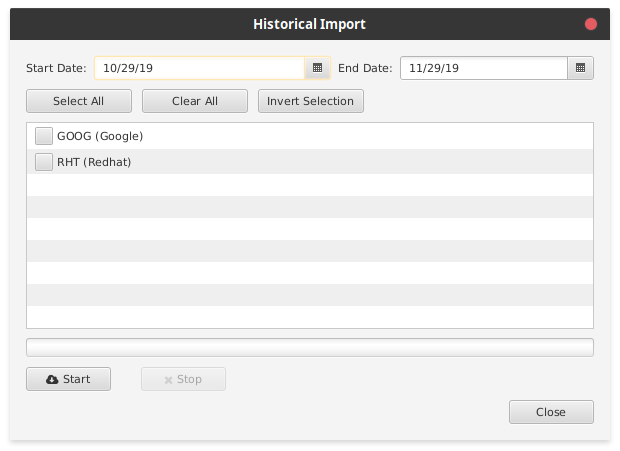
\includegraphics[width=1.0\linewidth]{images/securityHistoryImport}
    \end{figure}
          
    \subsection{Price Lookup and Reporting}
    \label{sec:pricelookup}
           
    When reporting balances for \hyperref[sub:investaccount]{Investment Accounts}, jGnash will perform a search
    for the most recent or closet price.
        
    \begin{itemize}
        \item If an Investment Transaction occurs on the same day as a price record, the Transaction price will be used.
        \item For reporting periods such as Months or Quarters, the closest or exact match to the end of the period is used.
        \item  In all cases, the latest price if it's a Transaction or a Historical record is used for the last period 
        of a Report and as well as the reported \textbf{Market Value} of the account shown in the Register.      
    \end{itemize}
      
    Deleting price records near the end of a reporting period can skew the reported interim values.

    \chapter{Importing Transactions}
    Importing of OFX, QFX, MT940, and QIF transaction files is supported within jGnash.
    The files are downloaded manually from your financial institution and then imported.
    jGnash does not currently support an automatic download process.

    QIF is an old format that was not well defined and is generated inconsistently between financial institutions.
    There are two significantly different formats with one consisting of transnational data only and the other format
    attempts to serve as an export / import format with account information for financial applications.
    Use of date formats within the QIF format will vary and can lead to incorrect or failed import of transactions.
    If at all possible, avoid use of QIF files and use an OFX or QFX file.

    OFX and QFX files are a well defined standard and jGnash will easily process these.
    This is the preferred file format for importing transactions into jGnash.
    OFX and QFX files are XML based and human readable in that you can open the file
    with a text editor and easily understand the information contained within.

    MT940 is another well defined standard commonly used between financial institutions.
    The format consists of fields separated by colons and commas with well defined numeric codes.
    MT940 is very compact and efficient to transfer electronically.

    \notebox{
    The Import Process below describes the basic import of transactions.
    jGnash can also process OFX and QFX files with Investment transactions.
    Additional columns will be present and enabled when applicable for these advanced types of transactions.
    }

    \section{Import Process}
    Importing transactions is an easy process that is guided with a simple wizard.
    It begins with \menu{File > Import > OFX / QFX}, \menu{File > Import > QIF}, or
    \menu{File > Import > MT940} and selecting a file that has been downloaded.

    The first step of the import process requires selecting the correct account the
    import file is for. This is the base account all imported transactions will be
    associated with.

    \tipbox{
    When importing OFX or QFX files, jGnash will preselect the correct account after
    it has learned from the first import.
    }

    The second step of the process is reviewing the transactions as shown below.

    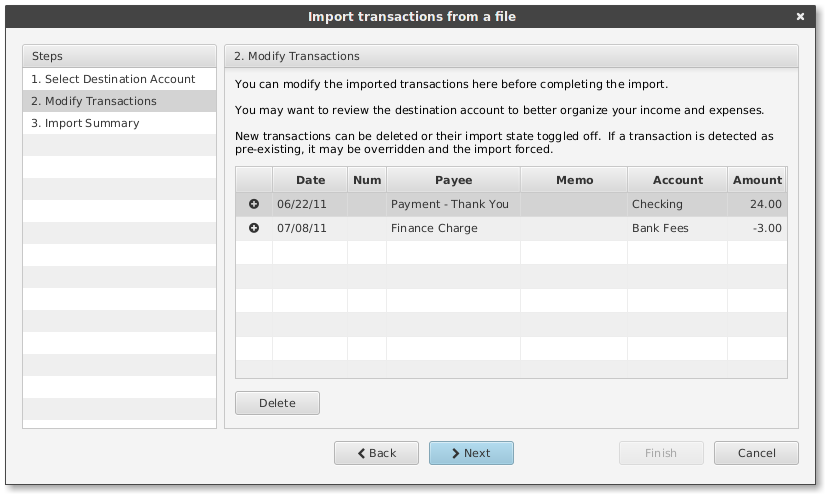
\includegraphics[width=0.8\linewidth]{images/importWizard2}

    The first column consists of import status symbols:

    \begin{itemize}
        \item A plus symbol indicates the transaction has been detected as new. Double
        clicking on it will change it to a negative symbol to indicate you do not want
        it to be imported.
        \item An equals symbol indicates the transaction has been detected as a duplicate of
        a manually entered transaction or already imported transaction. Double
        clicking on it will change it to a plus symbol to indicate you want to force
        the import of the transaction.
    \end{itemize}

    The second, third, and forth columns are not editable. The Payee and Memo
    columns may be pre-processed using JavaScript Filters as described later.

    The Account column can be double clicked and changed to suit. The selected
    account will normally be an income or expense account unless it was a transfer
    to another bank account or financial institution. This column is also the
    equivalent to \textit{Categories} for some other financial applications.

    The Amount column can be double clicked and edited. This is normally not
    needed and not recommended, but allowed for some specialized uses when working
    with multiple currencies.

    The \menu{Delete} button may also be used to remove a transaction being imported.

    \tipbox{
    When importing transactions, jGnash uses what is called a Naive Bayes Classifier
    to help preselect the best account for the transaction. Consistent use of
    memo and payee fields will help accuracy of account selection. Accuracy also
    improves with increased quantity of transactions over time.
    }

    The last step of the Import Wizard allows you to review basic information about
    the import before committing to the changes. After clicking on \menu{Finish},
    the dialog will close and jGnash will begin the import process.

    \section{OFX imports}
    Taking the time to correctly configure your jGnash Account properties can help
    reduce the effort needed to automatically identify Accounts when importing OFX
    transactions.

    OFX files may contain enough information to identify transfers between accounts.
    Most financial institutions will correctly identify transactions between checking
    and savings accounts with the bank, but others may include enough information
    when transferring between finance institutions.

    Below is a fragment of the OFX file content defining the transfer. jGnash will
    attempt to match the \texttt{<ACCTID>} identifier on line 4 to an existing Account Number
    that is specified within the properties of your jGnash account.
    \\ % new line
    \begin{lstlisting}[caption={OFX File Fragment}]
        <BANKACCTTO>
        <BANKID>100000009
        <BRANCHID>TEST
        <ACCTID>555555-C01
        <ACCTTYPE>CHECKING
        </BANKACCTTO>
    \end{lstlisting}

    The \textbf{Account Number} is easily changed by modifying the Account properties as described
    in the \hyperref[subsec:creatingAccounts]{Creating Accounts} section of the manual.

    \section{JavaScript Filters}
    When importing transactions from OFX/QFX, mt940, and QIF bank statements
    downloads, transactions may be preprocessed using custom JavaScript files. As
    of jGnash release 2.32.0, the scripts may be used to alter the memo or payee of
    the transactions being imported.

    You have three options for making a JavaScript file available for use:
    \begin{itemize}
        \item Some scripts are included by default. These show up as \texttt{/jgnash/imports/xxx.js}
        in the \textbf{Script} column of the table.
        \item Place the JavaScript file into a \directory{importScripts} sub directory where
        your jGnash data file is installed.
        \item Place the \texttt{.js} file into your home directly where jGnash will find it.
        \begin{itemize}
            \item \directory{\$HOME/.jgnash/importScripts} for UNIX and BSD based operating systems
            \item \directory{USER\_HOME\textbackslash AppData\textbackslash Local\textbackslash jgnash\textbackslash importScripts} for Windows operating systems.
        \end{itemize}
    \end{itemize}

    These import scripts must be specifically enabled for use and the order in which they will be executed can be changed
    using the \menu{Tools > Configure Transaction Imports Filters…} menu as shown below.

    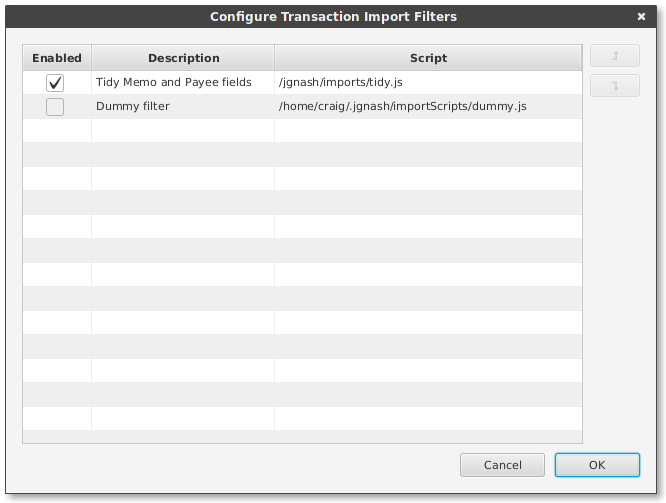
\includegraphics[width=0.9\linewidth]{images/importFilters}

    \newpage
    Below is an example JavaScript file. The first four functions are required for correct operation.

    The first function accepts an \textbf{ImportTransaction} for advanced manipulation of the imported data.

    The second and third functions accept a \textbf{string} and are expected to return a \textbf{string}.

    The \textbf{getDescription} function should return a meaningful description of the script.
    \\ % new line
    \begin{lstlisting}[caption={Example Import Script},language=JavaScript,numbers=left]
        /* Normalizes the case of the payee and memo fields */

        // place holder for the passed ImportTransaction
        var importTransaction;

        // This will be called first and passed the ImportTransaction
        function acceptTransaction(transaction) {

            // does nothing with it in this script
            importTransaction = transaction;
        }

        // This is a required function
        function processMemo(memo) {
            return capitalizeFirstLetter(memo.toLocaleLowerCase());
        }

        // This is a required function
        function processPayee(payee) {
            return titleCase(payee.toLocaleLowerCase());
        }

        // This is a required function
        var getDescription = function (locale) {
            var Locale = Packages.java.util.Locale;
    
            switch (locale) {
                case Locale.ENGLISH:
                    return "Tidy Memo and Payee fields";
                default:
                    return "Tidy Memo and Payee fields";
            }
        };

        // Capitalizes the first letter or a String
        function capitalizeFirstLetter(str) {
            return str.charAt(0).toUpperCase() + str.slice(1);
        }

        // Converts a string to Title Case
        function titleCase(str) {
            return str.replace(/(^|\s)[a-z]/g,function(f){return f.toUpperCase();});
        }
    \end{lstlisting}

    The full jGnash API may be accessed within these scripts for advanced processing capabilities.
    See the \hyperref[sec:javascript]{JavaScript} section of the manual for more details.

    \notebox{
    JavaScript files are expected to be encoded as UTF-8 Files.
    An incorrect file encoding may cause script failures.
    }

    \chapter{Reports}
    A variety of reports exist that present your financial history and status in different ways.
    There are currently three classes of reports available.
    Text reports can be exported and easily imported into a spreadsheet for advanced manipulation.
    Chart based reports may be altered and exported to a graphic file or printed using the context sensitive pop-up menu.
    Tabular type reports may be printed or saved as \textit{PDF}, \textit{XLS}, or \textit{XLSX} files.

    \section{Tabular Reports}
    Tabular reports are displayed in a viewer that allows you to change the page and print or export the report.
    The font size of the displayed report can be changed from the toolbar of the report window.

    The fonts used to display the report may be changed in the \menu{Tools > Options}
    dialog shown below. The \textbf{Proportional} font is typically used for report headers and footers.
    The \textbf{ Monospace} font, also called a fixed-width font, is used to display the reported values.

    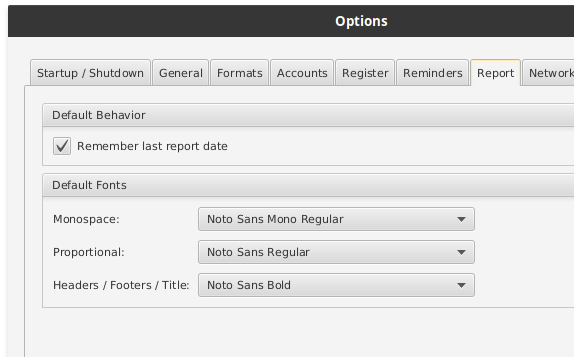
\includegraphics[width=0.6\linewidth]{images/font-options.png}

    If a proportional spaced font is chosen for the \textbf{ Monospace} font, numeric report values may not line up
    correctly in the report.

    \tipbox{
    Information on font types as well as a wide selection of freely available fonts can be found on the Internet.
    Once a new font is properly installed in your operating system, it will be available for use in jGnash the next
    time it is started.
    }

    \section{Tips}
    Depending on your operating system, or locale you may need to change the font type and font size to achieve
    the best looking report.
    The font size can be changed on the report toolbar and is remember for each report type.

    \subsection{Nothing displays in the report and I'm not getting any errors}
    Try increasing your font size, and if that does not work, choose a different font.
    Depending on your operation system, fonts may not render correctly at reduced sizes.

    \subsection{I get an error that tells me to reduce my font size}
    The selected font size is too large to display the report correctly.
    You will need to choose a smaller font size.
    Many times, the column heading text may dictate the displayed width of a column.
    Try choosing a proportional font with condensed spacing.
    You may also want to check the default paper size and adjust if needed.

    \subsection{My PDF exports are missing information or don't look correct on different computers}
    Not all fonts are able to be embedded within a \texttt{PDF} file.
    You may need to experiment with different fonts to achieve good portability.
    In most cases, the defaults jGnash chooses will give you good results.

    \subsection{The IRR is not being displayed in my Portfolio report}
    Your investment account may not be setup properly. Ensure that stocks have been added
    or purchased prior to sells, buys, dividends, etc.

    \chapter{Administration}
    Several administration options and tools are provided to help with management of your data.

    \section{File | Save As}
    An open file may be saved as a new file of the same type, or a new file with a new file type.
    To save the file as a different type, you must change the file extension to a supported type.
    Correct file extensions are shown below.

    \begin{table}[H]
        \begin{tabular}{|l|l|}
            \hline
            XML File & .xml \\
            \hline
            Binary File & .bxds \\
            \hline
            H2 Relational Database (B-Tree) & .h2.db \\
            \hline
            H2 Relational Database (MVStore) & .mv.db \textit{(newest H2 format and is more compact)} \\
            \hline
            HyperSql (hslqb) Relational Database & .script \textit{(.lobs, .log, .properties are used as support files)} \\
            \hline
        \end{tabular}
        \caption{File Types}
    \end{table}

    Depending on the file type, jGnash may generate an intermediate file for the conversion process.
    When saving to a relational database, the process may take awhile to complete.

    \section{File | Export | Export Accounts and File | Import | Import Accounts}
    Use of these commands allows you to export your account structure and import it back into and new file.
    This is handy if you want to start a new file without manually recreating your accounts.
    This does not preserve existing transactions.

    \section{Change Database Password}
    By default, when a new relational database is created, a password is not specified. This allows you to password protect
    your file. This does not encrypt your data, so a person with the right tools can \underline{easily} access your data.
    It is useful for casual protection only. If encryption is important, use OS level encryption capability available on
    any modern operating system. This is disabled while a file is open.

    \section{Shutdown Server}
    Issues a shutdown request to a remote server.
    This is disabled while a file is open.


    \chapter{Plugins and JavaScript}
    jGnash support the addition of JavaScript and Plugins to add additional functionality to the application.

    \section{Plugins}
    Plugins are tightly integrated into jGnash, and once loaded, behave as if they are a standard part of the application.
    Plugins are coded in Java using a jGnash specific API as the entry point so they may be loaded into jGnash.

    Standard Plugins are packaged into \texttt{JAR} files and are typically located within the \directory{plugins}
    directory located in the directory jGnash is installed.

    You have two options for manually installing a Plugin:
    \begin{itemize}
        \item Place the JAR file into the \directory{plugins} sub directory where jGnash is installed and restart jGnash.
        \item Place the JAR file into your home directly where jGnash will find it.
        \begin{itemize}
            \item \directory{\$HOME/.jgnash/plugins} for UNIX and BSD based operating systems.
            \item \directory{USER\_HOME\textbackslash AppData\textbackslash Local\textbackslash jgnash\textbackslash plugins} for Windows operating systems.
        \end{itemize}
    \end{itemize}

    The jGnash JavaDoc may be referenced if you are interested in creating a jGnash Plugin.
    The MT940 import is written as a standard Plugin and may be referenced as an example of how to write one.

    \section{JavaScript}
    \label{sec:javascript}

    In addition to use of Plugins, jGnash allows you to create and run JavaScript programs.
    The internals of the jGnash engine and some user interface functions can be accessed to create custom reports, create
    and modify transactions, etc.

    Running a JavaScript program is as simple as using \menu{Tools > Run JavaScript} command from the menu bar.

    Below is an example JavaScript program that displays the accounts in the currently loaded file and demonstrates how to
    display a simple dialog.
    To try the program, create a text file using your favorite editor with a name of your choice that ends with
    a \texttt{.js} extension.
    After creating the file, simply using the \menu{Tools > Run JavaScript} command to select the program and run it.
    \\
    \begin{lstlisting}[language=JavaScript,numbers=left]
        load("nashorn:mozilla_compat.js"); // Load compatibility script

        importPackage(javax.swing);
        importPackage(Packages.jgnash.ui);
        importPackage(Packages.jgnash.engine);

        // helper function to print messages to the console
        function debug(message) {
            java.lang.System.out.println(message);
        }

        // show the console dialog to see the debug information
        var Console = Java.type("jgnash.uifx.views.main.ConsoleDialogController");
        Console.show();

        // this is how to get the default Engine instance
        var engine = EngineFactory.getEngine(EngineFactory.DEFAULT);

        // get a list of accounts
        var accountList = engine.getAccountList();

        // loop and print the account names to the console
        for (var i = 0; i; accountList.size(); i++)
        {
            var account = accountList.get(i);
            debug(account.getName());
        }
    \end{lstlisting}

    \notebox{
    JavaScript files are expected to be encoded as UTF-8 Files. An incorrect file encoding may cause script failures.
    }

    JavaScript programs have the advantage of not requiring the use of an IDE or Java compiler to create and test a program.
    The disadvantage is troubleshooting syntax and logic errors can be more difficult than writing a jGnash Plugin.

    % ======================
    % Command Line Options
    % ======================
    \chapter{Command Line Options}
    \label{ch:cmdOptions}

    jGnash has several command line options for advanced users.

    Parameters such as file names that include a space in the path must be escaped using double quotes.

    \begin{mdframed}[style=info]
        \textbf{Example} \\ \\
        The path to the file "/home/craig/jgnash files/jgnash.h2.db" must be escaped as shown.
        \\ \\
        \texttt{jGnash -{}-server "/home/craig/jgnash files/jgnash.h2.db" -{}-password fh56dy}
    \end{mdframed}

    \section{Options}
    \begin{description}
        \item[-h, -{}-help]
        Detailed display of all command line options.
        \item[-f, -{}-file \textit{filename}]
        Specifies a file to load at startup.
        \item[-p, -{}-portable]
        If portable is specified on the command line, jGnash preferences will be stored to a file name \texttt{pref.xml}
        instead of using the system registry.
        Use of this option is intended for users who want to run jGnash from a thumb drive on multiple computers and
        maintain their preferences without using the system registry.
        The \texttt{pref.xml} file will usually be stored at the location jGnash was started from.
        \item[-{}-portableFile \textit{filename}]
        If you don't like the location the \texttt{pref.xml} file is stored, or wish to use a different name, use
        this option to change the location and name to suit.
        \item[-{}-bypassBootloader]
        Bypasses the boot loader and requires manual installation of any OS specific files.
        \item[-u, -{}-uninstall]
        Removes all registry and configuration settings jGnash has created.
        This will not have any effect if you have been using the \texttt{--portable} option.
    \end{description}

    \section{Client/Server Options}
    \begin{description}
        \item[-{}-server \textit{filename}]
        Starts the jGnash server using the specified file which must be must be a jGnash relational database.
        The file must exist and not be in use by another program.
        A user interface will not be displayed.
        \item[-{}-host \textit{servername}]
        Specifies the name of the remote server.
        This starts jGnash and automatically connects to the specified server.
        If running on the same computer as the server, \texttt{localhost} may be used as the name of the server.
        \item[-{}-shutdown]
        Issues a shutdown request to a server.
        If -{}-host is not specified, then \texttt{localhost} is assumed for the server name
        \item[-{}-password \textit{password}]
        The password that the client must correctly specify to connect to the jGnash database.
        This is not required if the database is not protected.
        A password does nothing to encrypt a file.
        \item[-{}-port \textit{port}]
        An empty port for network communications.
        The specified port and \texttt{port+1} may not be used by any other application at the same time.
        The default port is 5300.
    \end{description}

    \notebox{
    It is possible to start the jGnash client and specify the server, and password settings from
    the \menu{File > Open} dialog.
    }
    \newpage
    \section{Client/Server Examples}
    Start the jGnash server using the default port with a password protected database
    \begin{mdframed}[style=info]
        \texttt{jGnash -{}-server "/home/craig/jgnash.mv.db" -{}-password fh56dy}
    \end{mdframed}

    Start the jGnash client and connect to the local server running a password protected database
    \begin{mdframed}[style=info]
        \texttt{jGnash -{}-host localhost -{}-password fh56dy}
    \end{mdframed}

    Issue a shutdown request to a remote server that is password protected
    \begin{mdframed}[style=info]
        \texttt{jGnash -{}-shutdown -{}-host serv1 -{}-password fh56dy}
    \end{mdframed}


    Issue a shutdown request to a local server that is not password protected
    \begin{mdframed}[style=info]
        \texttt{jGnash -{}-shutdown}
    \end{mdframed}

    \chapter{Frequently Asked Questions}\label{ch:frequently-asked-questions}

    \begin{description}
        \item[Where do I set my opening account balance?]
        Create an Equity Account called "Opening Balances" and transfer money from the Equity account to they
        new account which will establish an opening balance.
        The "Opening Balances" account may be hidden later if you do not want it visible.
        \item[What happened to transaction categories?]
        Most commercial personal finance applications use categories to help track spending and income.
        jGnash uses Income and Expense accounts instead of categories for tracking where your money
        comes from and where it goes.
        \item[Can I use multiple currencies?]
        Yes, the \menu{Tool > Currencies > Add/Remove} menu will let you add additional currencies.
        \\ \\
        After adding new currencies, simple create new accounts that use the new currency.
        When creating a transaction between accounts with different currencies, a field for the exchange rate will be enabled.
        \item[How do I add Securities / Stocks to my Investment and Mutual Fund Account?]
        First, you need to have created your stocks/securities. \menu{Tools > Commodities > Create / Modify}.
        \\ \\
        When creating the securities, the scale field must be filled in and the prefix field should be filled in.
        The scale will generally be the same scale as the currency the securities value is reported in.
        In most cases, a scale of 2 will work fine.
        For the prefix, the currency prefix of the reported value should be used.
        \\ \\
        After creating your securities, you can go back and modify the existing account or select the securities when
        creating a new account.
        Use the \menu{Securities} button in the dialog to make changes.
    \end{description}
    \begin{appendices}
        \chapter{Keyboard Shortcuts}\label{ch:keyboard-shortcuts}
        This Appendix contains application keyboard shortcuts that are available to you throughout jGnash

        Depending on your operating system and how you have it configured, other shortcuts may be
        available that perform the same function.
        
        \begin{table}[H]
            \begin{tabular}{|l|l|}
                \hline
                \textbf{Keys} & \textbf{Function} \\
                \hline
                \hline
                \keys{CTRL + F4}& Closes the active register window if you have one open \\
                \hline
                \keys{CTRL + A} & Displays the About dialog \textit{(When a register table does not have the focus)}\\
                \hline
                \keys{CTRL + A} & Selects all transactions \textit{(When a register table has the focus)}\\
                \hline
                \keys{CTRL + C} & Copies selected transaction information to the clipboard \\
                \hline
            \end{tabular}
            \caption{Shortcut Keys}
        \end{table}

        \begin{table}[H]
            \begin{tabular}{|l|l|}
                \hline
                \textbf{Keys} & \textbf{Function} \\
                \hline
                \hline
                \keys{CTRL + C} & Copy \\
                \hline
                \keys{CTRL + X} & Cut \\
                \hline
                \keys{CTRL + V} & Paste \\
                \hline
            \end{tabular}
            \caption{Editing Keys}
        \end{table}

        \chapter{GNU General Public License}
\begin{center}
    Version 3, 29 June 2007 
\end{center}
Copyright \copyright\  2007 Free Software Foundation, Inc. \texttt{https://fsf.org/}

\bigskip
Everyone is permitted to copy and distribute verbatim copies of this
license document, but changing it is not allowed.

\section*{Preamble}
The GNU General Public License is a free, copyleft license for
software and other kinds of works.

The licenses for most software and other practical works are designed
to take away your freedom to share and change the works.  By contrast,
the GNU General Public License is intended to guarantee your freedom to
share and change all versions of a program--to make sure it remains free
software for all its users.  We, the Free Software Foundation, use the
GNU General Public License for most of our software; it applies also to
any other work released this way by its authors.  You can apply it to
your programs, too.

When we speak of free software, we are referring to freedom, not
price.  Our General Public Licenses are designed to make sure that you
have the freedom to distribute copies of free software (and charge for
them if you wish), that you receive source code or can get it if you
want it, that you can change the software or use pieces of it in new
free programs, and that you know you can do these things.

To protect your rights, we need to prevent others from denying you
these rights or asking you to surrender the rights.  Therefore, you have
certain responsibilities if you distribute copies of the software, or if
you modify it: responsibilities to respect the freedom of others.

For example, if you distribute copies of such a program, whether
gratis or for a fee, you must pass on to the recipients the same
freedoms that you received.  You must make sure that they, too, receive
or can get the source code.  And you must show them these terms so they
know their rights.

Developers that use the GNU GPL protect your rights with two steps:
(1) assert copyright on the software, and (2) offer you this License
giving you legal permission to copy, distribute and/or modify it.

For the developers' and authors' protection, the GPL clearly explains
that there is no warranty for this free software.  For both users' and
authors' sake, the GPL requires that modified versions be marked as
changed, so that their problems will not be attributed erroneously to
authors of previous versions.

Some devices are designed to deny users access to install or run
modified versions of the software inside them, although the manufacturer
can do so.  This is fundamentally incompatible with the aim of
protecting users' freedom to change the software.  The systematic
pattern of such abuse occurs in the area of products for individuals to
use, which is precisely where it is most unacceptable.  Therefore, we
have designed this version of the GPL to prohibit the practice for those
products.  If such problems arise substantially in other domains, we
stand ready to extend this provision to those domains in future versions
of the GPL, as needed to protect the freedom of users.

Finally, every program is threatened constantly by software patents.
States should not allow patents to restrict development and use of
software on general-purpose computers, but in those that do, we wish to
avoid the special danger that patents applied to a free program could
make it effectively proprietary.  To prevent this, the GPL assures that
patents cannot be used to render the program non-free.

The precise terms and conditions for copying, distribution and
modification follow.

\section*{Terms and Conditions}

\begin{enumerate}

\addtocounter{enumi}{-1}

\item Definitions.

``This License'' refers to version 3 of the GNU General Public License.

``Copyright'' also means copyright-like laws that apply to other kinds of
works, such as semiconductor masks.

``The Program'' refers to any copyrightable work licensed under this
License.  Each licensee is addressed as ``you''.  ``Licensees'' and
``recipients'' may be individuals or organizations.

To ``modify'' a work means to copy from or adapt all or part of the work
in a fashion requiring copyright permission, other than the making of an
exact copy.  The resulting work is called a ``modified version'' of the
earlier work or a work ``based on'' the earlier work.

A ``covered work'' means either the unmodified Program or a work based
on the Program.

To ``propagate'' a work means to do anything with it that, without
permission, would make you directly or secondarily liable for
infringement under applicable copyright law, except executing it on a
computer or modifying a private copy.  Propagation includes copying,
distribution (with or without modification), making available to the
public, and in some countries other activities as well.

To ``convey'' a work means any kind of propagation that enables other
parties to make or receive copies.  Mere interaction with a user through
a computer network, with no transfer of a copy, is not conveying.

An interactive user interface displays ``Appropriate Legal Notices''
to the extent that it includes a convenient and prominently visible
feature that (1) displays an appropriate copyright notice, and (2)
tells the user that there is no warranty for the work (except to the
extent that warranties are provided), that licensees may convey the
work under this License, and how to view a copy of this License.  If
the interface presents a list of user commands or options, such as a
menu, a prominent item in the list meets this criterion.

\item Source Code.

The ``source code'' for a work means the preferred form of the work
for making modifications to it.  ``Object code'' means any non-source
form of a work.

A ``Standard Interface'' means an interface that either is an official
standard defined by a recognized standards body, or, in the case of
interfaces specified for a particular programming language, one that
is widely used among developers working in that language.

The ``System Libraries'' of an executable work include anything, other
than the work as a whole, that (a) is included in the normal form of
packaging a Major Component, but which is not part of that Major
Component, and (b) serves only to enable use of the work with that
Major Component, or to implement a Standard Interface for which an
implementation is available to the public in source code form.  A
``Major Component'', in this context, means a major essential component
(kernel, window system, and so on) of the specific operating system
(if any) on which the executable work runs, or a compiler used to
produce the work, or an object code interpreter used to run it.

The ``Corresponding Source'' for a work in object code form means all
the source code needed to generate, install, and (for an executable
work) run the object code and to modify the work, including scripts to
control those activities.  However, it does not include the work's
System Libraries, or general-purpose tools or generally available free
programs which are used unmodified in performing those activities but
which are not part of the work.  For example, Corresponding Source
includes interface definition files associated with source files for
the work, and the source code for shared libraries and dynamically
linked subprograms that the work is specifically designed to require,
such as by intimate data communication or control flow between those
subprograms and other parts of the work.

The Corresponding Source need not include anything that users
can regenerate automatically from other parts of the Corresponding
Source.

The Corresponding Source for a work in source code form is that
same work.

\item Basic Permissions.

All rights granted under this License are granted for the term of
copyright on the Program, and are irrevocable provided the stated
conditions are met.  This License explicitly affirms your unlimited
permission to run the unmodified Program.  The output from running a
covered work is covered by this License only if the output, given its
content, constitutes a covered work.  This License acknowledges your
rights of fair use or other equivalent, as provided by copyright law.

You may make, run and propagate covered works that you do not
convey, without conditions so long as your license otherwise remains
in force.  You may convey covered works to others for the sole purpose
of having them make modifications exclusively for you, or provide you
with facilities for running those works, provided that you comply with
the terms of this License in conveying all material for which you do
not control copyright.  Those thus making or running the covered works
for you must do so exclusively on your behalf, under your direction
and control, on terms that prohibit them from making any copies of
your copyrighted material outside their relationship with you.

Conveying under any other circumstances is permitted solely under
the conditions stated below.  Sublicensing is not allowed; section 10
makes it unnecessary.

\item Protecting Users' Legal Rights From Anti-Circumvention Law.

No covered work shall be deemed part of an effective technological
measure under any applicable law fulfilling obligations under article
11 of the WIPO copyright treaty adopted on 20 December 1996, or
similar laws prohibiting or restricting circumvention of such
measures.

When you convey a covered work, you waive any legal power to forbid
circumvention of technological measures to the extent such circumvention
is effected by exercising rights under this License with respect to
the covered work, and you disclaim any intention to limit operation or
modification of the work as a means of enforcing, against the work's
users, your or third parties' legal rights to forbid circumvention of
technological measures.

\item Conveying Verbatim Copies.

You may convey verbatim copies of the Program's source code as you
receive it, in any medium, provided that you conspicuously and
appropriately publish on each copy an appropriate copyright notice;
keep intact all notices stating that this License and any
non-permissive terms added in accord with section 7 apply to the code;
keep intact all notices of the absence of any warranty; and give all
recipients a copy of this License along with the Program.

You may charge any price or no price for each copy that you convey,
and you may offer support or warranty protection for a fee.

\item Conveying Modified Source Versions.

You may convey a work based on the Program, or the modifications to
produce it from the Program, in the form of source code under the
terms of section 4, provided that you also meet all of these conditions:
  \begin{enumerate}
  \item The work must carry prominent notices stating that you modified
  it, and giving a relevant date.

  \item The work must carry prominent notices stating that it is
  released under this License and any conditions added under section
  7.  This requirement modifies the requirement in section 4 to
  ``keep intact all notices''.

  \item You must license the entire work, as a whole, under this
  License to anyone who comes into possession of a copy.  This
  License will therefore apply, along with any applicable section 7
  additional terms, to the whole of the work, and all its parts,
  regardless of how they are packaged.  This License gives no
  permission to license the work in any other way, but it does not
  invalidate such permission if you have separately received it.

  \item If the work has interactive user interfaces, each must display
  Appropriate Legal Notices; however, if the Program has interactive
  interfaces that do not display Appropriate Legal Notices, your
  work need not make them do so.
\end{enumerate}
A compilation of a covered work with other separate and independent
works, which are not by their nature extensions of the covered work,
and which are not combined with it such as to form a larger program,
in or on a volume of a storage or distribution medium, is called an
``aggregate'' if the compilation and its resulting copyright are not
used to limit the access or legal rights of the compilation's users
beyond what the individual works permit.  Inclusion of a covered work
in an aggregate does not cause this License to apply to the other
parts of the aggregate.

\item Conveying Non-Source Forms.

You may convey a covered work in object code form under the terms
of sections 4 and 5, provided that you also convey the
machine-readable Corresponding Source under the terms of this License,
in one of these ways:
  \begin{enumerate}
  \item Convey the object code in, or embodied in, a physical product
  (including a physical distribution medium), accompanied by the
  Corresponding Source fixed on a durable physical medium
  customarily used for software interchange.

  \item Convey the object code in, or embodied in, a physical product
  (including a physical distribution medium), accompanied by a
  written offer, valid for at least three years and valid for as
  long as you offer spare parts or customer support for that product
  model, to give anyone who possesses the object code either (1) a
  copy of the Corresponding Source for all the software in the
  product that is covered by this License, on a durable physical
  medium customarily used for software interchange, for a price no
  more than your reasonable cost of physically performing this
  conveying of source, or (2) access to copy the
  Corresponding Source from a network server at no charge.

  \item Convey individual copies of the object code with a copy of the
  written offer to provide the Corresponding Source.  This
  alternative is allowed only occasionally and noncommercially, and
  only if you received the object code with such an offer, in accord
  with subsection 6b.

  \item Convey the object code by offering access from a designated
  place (gratis or for a charge), and offer equivalent access to the
  Corresponding Source in the same way through the same place at no
  further charge.  You need not require recipients to copy the
  Corresponding Source along with the object code.  If the place to
  copy the object code is a network server, the Corresponding Source
  may be on a different server (operated by you or a third party)
  that supports equivalent copying facilities, provided you maintain
  clear directions next to the object code saying where to find the
  Corresponding Source.  Regardless of what server hosts the
  Corresponding Source, you remain obligated to ensure that it is
  available for as long as needed to satisfy these requirements.

  \item Convey the object code using peer-to-peer transmission, provided
  you inform other peers where the object code and Corresponding
  Source of the work are being offered to the general public at no
  charge under subsection 6d.
  \end{enumerate}

A separable portion of the object code, whose source code is excluded
from the Corresponding Source as a System Library, need not be
included in conveying the object code work.

A ``User Product'' is either (1) a ``consumer product'', which means any
tangible personal property which is normally used for personal, family,
or household purposes, or (2) anything designed or sold for incorporation
into a dwelling.  In determining whether a product is a consumer product,
doubtful cases shall be resolved in favor of coverage.  For a particular
product received by a particular user, ``normally used'' refers to a
typical or common use of that class of product, regardless of the status
of the particular user or of the way in which the particular user
actually uses, or expects or is expected to use, the product.  A product
is a consumer product regardless of whether the product has substantial
commercial, industrial or non-consumer uses, unless such uses represent
the only significant mode of use of the product.

``Installation Information'' for a User Product means any methods,
procedures, authorization keys, or other information required to install
and execute modified versions of a covered work in that User Product from
a modified version of its Corresponding Source.  The information must
suffice to ensure that the continued functioning of the modified object
code is in no case prevented or interfered with solely because
modification has been made.

If you convey an object code work under this section in, or with, or
specifically for use in, a User Product, and the conveying occurs as
part of a transaction in which the right of possession and use of the
User Product is transferred to the recipient in perpetuity or for a
fixed term (regardless of how the transaction is characterized), the
Corresponding Source conveyed under this section must be accompanied
by the Installation Information.  But this requirement does not apply
if neither you nor any third party retains the ability to install
modified object code on the User Product (for example, the work has
been installed in ROM).

The requirement to provide Installation Information does not include a
requirement to continue to provide support service, warranty, or updates
for a work that has been modified or installed by the recipient, or for
the User Product in which it has been modified or installed.  Access to a
network may be denied when the modification itself materially and
adversely affects the operation of the network or violates the rules and
protocols for communication across the network.

Corresponding Source conveyed, and Installation Information provided,
in accord with this section must be in a format that is publicly
documented (and with an implementation available to the public in
source code form), and must require no special password or key for
unpacking, reading or copying.

\item Additional Terms.

``Additional permissions'' are terms that supplement the terms of this
License by making exceptions from one or more of its conditions.
Additional permissions that are applicable to the entire Program shall
be treated as though they were included in this License, to the extent
that they are valid under applicable law.  If additional permissions
apply only to part of the Program, that part may be used separately
under those permissions, but the entire Program remains governed by
this License without regard to the additional permissions.

When you convey a copy of a covered work, you may at your option
remove any additional permissions from that copy, or from any part of
it.  (Additional permissions may be written to require their own
removal in certain cases when you modify the work.)  You may place
additional permissions on material, added by you to a covered work,
for which you have or can give appropriate copyright permission.

Notwithstanding any other provision of this License, for material you
add to a covered work, you may (if authorized by the copyright holders of
that material) supplement the terms of this License with terms:
  \begin{enumerate}
  \item Disclaiming warranty or limiting liability differently from the
  terms of sections 15 and 16 of this License; or

  \item Requiring preservation of specified reasonable legal notices or
  author attributions in that material or in the Appropriate Legal
  Notices displayed by works containing it; or

  \item Prohibiting misrepresentation of the origin of that material, or
  requiring that modified versions of such material be marked in
  reasonable ways as different from the original version; or

  \item Limiting the use for publicity purposes of names of licensors or
  authors of the material; or

  \item Declining to grant rights under trademark law for use of some
  trade names, trademarks, or service marks; or

  \item Requiring indemnification of licensors and authors of that
  material by anyone who conveys the material (or modified versions of
  it) with contractual assumptions of liability to the recipient, for
  any liability that these contractual assumptions directly impose on
  those licensors and authors.
  \end{enumerate}

All other non-permissive additional terms are considered ``further
restrictions'' within the meaning of section 10.  If the Program as you
received it, or any part of it, contains a notice stating that it is
governed by this License along with a term that is a further
restriction, you may remove that term.  If a license document contains
a further restriction but permits relicensing or conveying under this
License, you may add to a covered work material governed by the terms
of that license document, provided that the further restriction does
not survive such relicensing or conveying.

If you add terms to a covered work in accord with this section, you
must place, in the relevant source files, a statement of the
additional terms that apply to those files, or a notice indicating
where to find the applicable terms.

Additional terms, permissive or non-permissive, may be stated in the
form of a separately written license, or stated as exceptions;
the above requirements apply either way.

\item Termination.

You may not propagate or modify a covered work except as expressly
provided under this License.  Any attempt otherwise to propagate or
modify it is void, and will automatically terminate your rights under
this License (including any patent licenses granted under the third
paragraph of section 11).

However, if you cease all violation of this License, then your
license from a particular copyright holder is reinstated (a)
provisionally, unless and until the copyright holder explicitly and
finally terminates your license, and (b) permanently, if the copyright
holder fails to notify you of the violation by some reasonable means
prior to 60 days after the cessation.

Moreover, your license from a particular copyright holder is
reinstated permanently if the copyright holder notifies you of the
violation by some reasonable means, this is the first time you have
received notice of violation of this License (for any work) from that
copyright holder, and you cure the violation prior to 30 days after
your receipt of the notice.

Termination of your rights under this section does not terminate the
licenses of parties who have received copies or rights from you under
this License.  If your rights have been terminated and not permanently
reinstated, you do not qualify to receive new licenses for the same
material under section 10.

\item Acceptance Not Required for Having Copies.

You are not required to accept this License in order to receive or
run a copy of the Program.  Ancillary propagation of a covered work
occurring solely as a consequence of using peer-to-peer transmission
to receive a copy likewise does not require acceptance.  However,
nothing other than this License grants you permission to propagate or
modify any covered work.  These actions infringe copyright if you do
not accept this License.  Therefore, by modifying or propagating a
covered work, you indicate your acceptance of this License to do so.

\item Automatic Licensing of Downstream Recipients.

Each time you convey a covered work, the recipient automatically
receives a license from the original licensors, to run, modify and
propagate that work, subject to this License.  You are not responsible
for enforcing compliance by third parties with this License.

An ``entity transaction'' is a transaction transferring control of an
organization, or substantially all assets of one, or subdividing an
organization, or merging organizations.  If propagation of a covered
work results from an entity transaction, each party to that
transaction who receives a copy of the work also receives whatever
licenses to the work the party's predecessor in interest had or could
give under the previous paragraph, plus a right to possession of the
Corresponding Source of the work from the predecessor in interest, if
the predecessor has it or can get it with reasonable efforts.

You may not impose any further restrictions on the exercise of the
rights granted or affirmed under this License.  For example, you may
not impose a license fee, royalty, or other charge for exercise of
rights granted under this License, and you may not initiate litigation
(including a cross-claim or counterclaim in a lawsuit) alleging that
any patent claim is infringed by making, using, selling, offering for
sale, or importing the Program or any portion of it.

\item Patents.

A ``contributor'' is a copyright holder who authorizes use under this
License of the Program or a work on which the Program is based.  The
work thus licensed is called the contributor's ``contributor version''.

A contributor's ``essential patent claims'' are all patent claims
owned or controlled by the contributor, whether already acquired or
hereafter acquired, that would be infringed by some manner, permitted
by this License, of making, using, or selling its contributor version,
but do not include claims that would be infringed only as a
consequence of further modification of the contributor version.  For
purposes of this definition, ``control'' includes the right to grant
patent sublicenses in a manner consistent with the requirements of
this License.

Each contributor grants you a non-exclusive, worldwide, royalty-free
patent license under the contributor's essential patent claims, to
make, use, sell, offer for sale, import and otherwise run, modify and
propagate the contents of its contributor version.

In the following three paragraphs, a ``patent license'' is any express
agreement or commitment, however denominated, not to enforce a patent
(such as an express permission to practice a patent or covenant not to
sue for patent infringement).  To ``grant'' such a patent license to a
party means to make such an agreement or commitment not to enforce a
patent against the party.

If you convey a covered work, knowingly relying on a patent license,
and the Corresponding Source of the work is not available for anyone
to copy, free of charge and under the terms of this License, through a
publicly available network server or other readily accessible means,
then you must either (1) cause the Corresponding Source to be so
available, or (2) arrange to deprive yourself of the benefit of the
patent license for this particular work, or (3) arrange, in a manner
consistent with the requirements of this License, to extend the patent
license to downstream recipients.  ``Knowingly relying'' means you have
actual knowledge that, but for the patent license, your conveying the
covered work in a country, or your recipient's use of the covered work
in a country, would infringe one or more identifiable patents in that
country that you have reason to believe are valid.

If, pursuant to or in connection with a single transaction or
arrangement, you convey, or propagate by procuring conveyance of, a
covered work, and grant a patent license to some of the parties
receiving the covered work authorizing them to use, propagate, modify
or convey a specific copy of the covered work, then the patent license
you grant is automatically extended to all recipients of the covered
work and works based on it.

A patent license is ``discriminatory'' if it does not include within
the scope of its coverage, prohibits the exercise of, or is
conditioned on the non-exercise of one or more of the rights that are
specifically granted under this License.  You may not convey a covered
work if you are a party to an arrangement with a third party that is
in the business of distributing software, under which you make payment
to the third party based on the extent of your activity of conveying
the work, and under which the third party grants, to any of the
parties who would receive the covered work from you, a discriminatory
patent license (a) in connection with copies of the covered work
conveyed by you (or copies made from those copies), or (b) primarily
for and in connection with specific products or compilations that
contain the covered work, unless you entered into that arrangement,
or that patent license was granted, prior to 28 March 2007.

Nothing in this License shall be construed as excluding or limiting
any implied license or other defenses to infringement that may
otherwise be available to you under applicable patent law.

\item No Surrender of Others' Freedom.

If conditions are imposed on you (whether by court order, agreement or
otherwise) that contradict the conditions of this License, they do not
excuse you from the conditions of this License.  If you cannot convey a
covered work so as to satisfy simultaneously your obligations under this
License and any other pertinent obligations, then as a consequence you may
not convey it at all.  For example, if you agree to terms that obligate you
to collect a royalty for further conveying from those to whom you convey
the Program, the only way you could satisfy both those terms and this
License would be to refrain entirely from conveying the Program.

\item Use with the GNU Affero General Public License.

Notwithstanding any other provision of this License, you have
permission to link or combine any covered work with a work licensed
under version 3 of the GNU Affero General Public License into a single
combined work, and to convey the resulting work.  The terms of this
License will continue to apply to the part which is the covered work,
but the special requirements of the GNU Affero General Public License,
section 13, concerning interaction through a network will apply to the
combination as such.

\item Revised Versions of this License.

The Free Software Foundation may publish revised and/or new versions of
the GNU General Public License from time to time.  Such new versions will
be similar in spirit to the present version, but may differ in detail to
address new problems or concerns.

Each version is given a distinguishing version number.  If the
Program specifies that a certain numbered version of the GNU General
Public License ``or any later version'' applies to it, you have the
option of following the terms and conditions either of that numbered
version or of any later version published by the Free Software
Foundation.  If the Program does not specify a version number of the
GNU General Public License, you may choose any version ever published
by the Free Software Foundation.

If the Program specifies that a proxy can decide which future
versions of the GNU General Public License can be used, that proxy's
public statement of acceptance of a version permanently authorizes you
to choose that version for the Program.

Later license versions may give you additional or different
permissions.  However, no additional obligations are imposed on any
author or copyright holder as a result of your choosing to follow a
later version.

\item Disclaimer of Warranty.

\begin{sloppypar}
 THERE IS NO WARRANTY FOR THE PROGRAM, TO THE EXTENT PERMITTED BY
 APPLICABLE LAW.  EXCEPT WHEN OTHERWISE STATED IN WRITING THE
 COPYRIGHT HOLDERS AND/OR OTHER PARTIES PROVIDE THE PROGRAM ``AS IS''
 WITHOUT WARRANTY OF ANY KIND, EITHER EXPRESSED OR IMPLIED,
 INCLUDING, BUT NOT LIMITED TO, THE IMPLIED WARRANTIES OF
 MERCHANTABILITY AND FITNESS FOR A PARTICULAR PURPOSE.  THE ENTIRE
 RISK AS TO THE QUALITY AND PERFORMANCE OF THE PROGRAM IS WITH YOU\@.
 SHOULD THE PROGRAM PROVE DEFECTIVE, YOU ASSUME THE COST OF ALL
 NECESSARY SERVICING, REPAIR OR CORRECTION\@.
\end{sloppypar}

\item Limitation of Liability.

 IN NO EVENT UNLESS REQUIRED BY APPLICABLE LAW OR AGREED TO IN
 WRITING WILL ANY COPYRIGHT HOLDER, OR ANY OTHER PARTY WHO MODIFIES
 AND/OR CONVEYS THE PROGRAM AS PERMITTED ABOVE, BE LIABLE TO YOU FOR
 DAMAGES, INCLUDING ANY GENERAL, SPECIAL, INCIDENTAL OR CONSEQUENTIAL
 DAMAGES ARISING OUT OF THE USE OR INABILITY TO USE THE PROGRAM
 (INCLUDING BUT NOT LIMITED TO LOSS OF DATA OR DATA BEING RENDERED
 INACCURATE OR LOSSES SUSTAINED BY YOU OR THIRD PARTIES OR A FAILURE
 OF THE PROGRAM TO OPERATE WITH ANY OTHER PROGRAMS), EVEN IF SUCH
 HOLDER OR OTHER PARTY HAS BEEN ADVISED OF THE POSSIBILITY OF SUCH
 DAMAGES\@.

\item Interpretation of Sections 15 and 16.

If the disclaimer of warranty and limitation of liability provided
above cannot be given local legal effect according to their terms,
reviewing courts shall apply local law that most closely approximates
an absolute waiver of all civil liability in connection with the
Program, unless a warranty or assumption of liability accompanies a
copy of the Program in return for a fee.

\begin{center}
{\Large\textsc{End of Terms and Conditions} }
\end{center}

\begin{center}
    {\Large\textbf{How to Apply These Terms to Your New Programs} }
\end{center}

If you develop a new program, and you want it to be of the greatest
possible use to the public, the best way to achieve this is to make it
free software which everyone can redistribute and change under these terms.

To do so, attach the following notices to the program.  It is safest
to attach them to the start of each source file to most effectively
state the exclusion of warranty; and each file should have at least
the ``copyright'' line and a pointer to where the full notice is found.

{\footnotesize
\begin{verbatim}
<one line to give the program's name and a brief idea of what it does.>

Copyright (C) <textyear>  <name of author>

This program is free software: you can redistribute it and/or modify
it under the terms of the GNU General Public License as published by
the Free Software Foundation, either version 3 of the License, or
(at your option) any later version.

This program is distributed in the hope that it will be useful,
but WITHOUT ANY WARRANTY; without even the implied warranty of
MERCHANTABILITY or FITNESS FOR A PARTICULAR PURPOSE.  See the
GNU General Public License for more details.

You should have received a copy of the GNU General Public License
along with this program.  If not, see <https://www.gnu.org/licenses/>.
\end{verbatim}
}

Also add information on how to contact you by electronic and paper mail.

If the program does terminal interaction, make it output a short
notice like this when it starts in an interactive mode:

{\footnotesize
\begin{verbatim}
<program>  Copyright (C) <year>  <name of author>

This program comes with ABSOLUTELY NO WARRANTY; for details type `show w'.
This is free software, and you are welcome to redistribute it
under certain conditions; type `show c' for details.
\end{verbatim}
}

The hypothetical commands {\texttt{show w} } and {\texttt{show c} } should show
the appropriate
parts of the General Public License.  Of course, your program's commands
might be different; for a GUI interface, you would use an ``about box''.

You should also get your employer (if you work as a programmer) or
school, if any, to sign a ``copyright disclaimer'' for the program, if
necessary.  For more information on this, and how to apply and follow
the GNU GPL, see \texttt{https://www.gnu.org/licenses/}.

The GNU General Public License does not permit incorporating your
program into proprietary programs.  If your program is a subroutine
library, you may consider it more useful to permit linking proprietary
applications with the library.  If this is what you want to do, use
the GNU Lesser General Public License instead of this License.  But
first, please read \texttt{https://www.gnu.org/licenses/why-not-lgpl.html}.

\end{enumerate}

%\end{document}


        \chapter{GNU Free Documentation License}
%\phantomsection  % so hyperref creates bookmarks
%\addcontentsline{toc}{chapter}{GNU Free Documentation License}


 \begin{center}
       Version 1.3, 3 November 2008

 Copyright \copyright{} 2000, 2001, 2002, 2007, 2008  Free Software Foundation, Inc.
 
 \bigskip 
     \texttt{<https://fsf.org/>}  
 \bigskip
 
 Everyone is permitted to copy and distribute verbatim copies
 of this license document, but changing it is not allowed.
\end{center}


\begin{center}
{\textbf{\large} Preamble}
\end{center}

The purpose of this License is to make a manual, textbook, or other
functional and useful document ``free'' in the sense of freedom: to
assure everyone the effective freedom to copy and redistribute it,
with or without modifying it, either commercially or noncommercially.
Secondarily, this License preserves for the author and publisher a way
to get credit for their work, while not being considered responsible
for modifications made by others.

This License is a kind of ``copyleft'', which means that derivative
works of the document must themselves be free in the same sense.  It
complements the GNU General Public License, which is a copyleft
license designed for free software.

We have designed this License in order to use it for manuals for free
software, because free software needs free documentation: a free
program should come with manuals providing the same freedoms that the
software does.  But this License is not limited to software manuals;
it can be used for any textual work, regardless of subject matter or
whether it is published as a printed book.  We recommend this License
principally for works whose purpose is instruction or reference.


\begin{center}
{\Large\textbf{1. APPLICABILITY AND DEFINITIONS} \par}
\end{center}

This License applies to any manual or other work, in any medium, that
contains a notice placed by the copyright holder saying it can be
distributed under the terms of this License.  Such a notice grants a
world-wide, royalty-free license, unlimited in duration, to use that
work under the conditions stated herein.  The ``\textbf{Document}'', below,
refers to any such manual or work.  Any member of the public is a
licensee, and is addressed as ``\textbf{you}''.  You accept the license if you
copy, modify or distribute the work in a way requiring permission
under copyright law.

A ``\textbf{Modified Version}'' of the Document means any work containing the
Document or a portion of it, either copied verbatim, or with
modifications and/or translated into another language.

A ``\textbf{Secondary Section}'' is a named appendix or a front-matter section of
the Document that deals exclusively with the relationship of the
publishers or authors of the Document to the Document's overall subject
(or to related matters) and contains nothing that could fall directly
within that overall subject.  (Thus, if the Document is in part a
textbook of mathematics, a Secondary Section may not explain any
mathematics.)  The relationship could be a matter of historical
connection with the subject or with related matters, or of legal,
commercial, philosophical, ethical or political position regarding
them.

The ``\textbf{Invariant Sections}'' are certain Secondary Sections whose titles
are designated, as being those of Invariant Sections, in the notice
that says that the Document is released under this License.  If a
section does not fit the above definition of Secondary then it is not
allowed to be designated as Invariant.  The Document may contain zero
Invariant Sections.  If the Document does not identify any Invariant
Sections then there are none.

The ``\textbf{Cover Texts}'' are certain short passages of text that are listed,
as Front-Cover Texts or Back-Cover Texts, in the notice that says that
the Document is released under this License.  A Front-Cover Text may
be at most 5 words, and a Back-Cover Text may be at most 25 words.

A ``\textbf{Transparent}'' copy of the Document means a machine-readable copy,
represented in a format whose specification is available to the
general public, that is suitable for revising the document
straightforwardly with generic text editors or (for images composed of
pixels) generic paint programs or (for drawings) some widely available
drawing editor, and that is suitable for input to text formatters or
for automatic translation to a variety of formats suitable for input
to text formatters.  A copy made in an otherwise Transparent file
format whose markup, or absence of markup, has been arranged to thwart
or discourage subsequent modification by readers is not Transparent.
An image format is not Transparent if used for any substantial amount
of text.  A copy that is not ``Transparent'' is called ``\textbf{Opaque}''.

Examples of suitable formats for Transparent copies include plain
ASCII without markup, Texinfo input format, LaTeX input format, SGML
or XML using a publicly available DTD, and standard-conforming simple
HTML, PostScript or PDF designed for human modification.  Examples of
transparent image formats include PNG, XCF and JPG.  Opaque formats
include proprietary formats that can be read and edited only by
proprietary word processors, SGML or XML for which the DTD and/or
processing tools are not generally available, and the
machine-generated HTML, PostScript or PDF produced by some word
processors for output purposes only.

The ``\textbf{Title Page}'' means, for a printed book, the title page itself,
plus such following pages as are needed to hold, legibly, the material
this License requires to appear in the title page.  For works in
formats which do not have any title page as such, ``Title Page'' means
the text near the most prominent appearance of the work's title,
preceding the beginning of the body of the text.

The ``\textbf{publisher}'' means any person or entity that distributes
copies of the Document to the public.

A section ``\textbf{Entitled XYZ}'' means a named subunit of the Document whose
title either is precisely XYZ or contains XYZ in parentheses following
text that translates XYZ in another language.  (Here XYZ stands for a
specific section name mentioned below, such as ``\textbf{Acknowledgements}'',
``\textbf{Dedications}'', ``\textbf{Endorsements}'', or ``\textbf{History}''.)  
To ``\textbf{Preserve the Title}''
of such a section when you modify the Document means that it remains a
section ``Entitled XYZ'' according to this definition.

The Document may include Warranty Disclaimers next to the notice which
states that this License applies to the Document.  These Warranty
Disclaimers are considered to be included by reference in this
License, but only as regards disclaiming warranties: any other
implication that these Warranty Disclaimers may have is void and has
no effect on the meaning of this License.


\begin{center}
{\Large\textbf{2. VERBATIM COPYING} \par}
\end{center}

You may copy and distribute the Document in any medium, either
commercially or noncommercially, provided that this License, the
copyright notices, and the license notice saying this License applies
to the Document are reproduced in all copies, and that you add no other
conditions whatsoever to those of this License.  You may not use
technical measures to obstruct or control the reading or further
copying of the copies you make or distribute.  However, you may accept
compensation in exchange for copies.  If you distribute a large enough
number of copies you must also follow the conditions in section~3.

You may also lend copies, under the same conditions stated above, and
you may publicly display copies.


\begin{center}
{\Large\textbf{3. COPYING IN QUANTITY} \par}
\end{center}


If you publish printed copies (or copies in media that commonly have
printed covers) of the Document, numbering more than 100, and the
Document's license notice requires Cover Texts, you must enclose the
copies in covers that carry, clearly and legibly, all these Cover
Texts: Front-Cover Texts on the front cover, and Back-Cover Texts on
the back cover.  Both covers must also clearly and legibly identify
you as the publisher of these copies.  The front cover must present
the full title with all words of the title equally prominent and
visible.  You may add other material on the covers in addition.
Copying with changes limited to the covers, as long as they preserve
the title of the Document and satisfy these conditions, can be treated
as verbatim copying in other respects.

If the required texts for either cover are too voluminous to fit
legibly, you should put the first ones listed (as many as fit
reasonably) on the actual cover, and continue the rest onto adjacent
pages.

If you publish or distribute Opaque copies of the Document numbering
more than 100, you must either include a machine-readable Transparent
copy along with each Opaque copy, or state in or with each Opaque copy
a computer-network location from which the general network-using
public has access to download using public-standard network protocols
a complete Transparent copy of the Document, free of added material.
If you use the latter option, you must take reasonably prudent steps,
when you begin distribution of Opaque copies in quantity, to ensure
that this Transparent copy will remain thus accessible at the stated
location until at least one year after the last time you distribute an
Opaque copy (directly or through your agents or retailers) of that
edition to the public.

It is requested, but not required, that you contact the authors of the
Document well before redistributing any large number of copies, to give
them a chance to provide you with an updated version of the Document.


\begin{center}
{\Large\textbf{4. MODIFICATIONS} \par}
\end{center}

You may copy and distribute a Modified Version of the Document under
the conditions of sections 2 and 3 above, provided that you release
the Modified Version under precisely this License, with the Modified
Version filling the role of the Document, thus licensing distribution
and modification of the Modified Version to whoever possesses a copy
of it.  In addition, you must do these things in the Modified Version:

\begin{itemize}
\item[A.] 
   Use in the Title Page (and on the covers, if any) a title distinct
   from that of the Document, and from those of previous versions
   (which should, if there were any, be listed in the History section
   of the Document).  You may use the same title as a previous version
   if the original publisher of that version gives permission.
   
\item[B.]
   List on the Title Page, as authors, one or more persons or entities
   responsible for authorship of the modifications in the Modified
   Version, together with at least five of the principal authors of the
   Document (all of its principal authors, if it has fewer than five),
   unless they release you from this requirement.
   
\item[C.]
   State on the Title page the name of the publisher of the
   Modified Version, as the publisher.
   
\item[D.]
   Preserve all the copyright notices of the Document.
   
\item[E.]
   Add an appropriate copyright notice for your modifications
   adjacent to the other copyright notices.
   
\item[F.]
   Include, immediately after the copyright notices, a license notice
   giving the public permission to use the Modified Version under the
   terms of this License, in the form shown in the Addendum below.
   
\item[G.]
   Preserve in that license notice the full lists of Invariant Sections
   and required Cover Texts given in the Document's license notice.
   
\item[H.]
   Include an unaltered copy of this License.
   
\item[I.]
   Preserve the section Entitled ``History'', Preserve its Title, and add
   to it an item stating at least the title, year, new authors, and
   publisher of the Modified Version as given on the Title Page.  If
   there is no section Entitled ``History'' in the Document, create one
   stating the title, year, authors, and publisher of the Document as
   given on its Title Page, then add an item describing the Modified
   Version as stated in the previous sentence.
   
\item[J.]
   Preserve the network location, if any, given in the Document for
   public access to a Transparent copy of the Document, and likewise
   the network locations given in the Document for previous versions
   it was based on.  These may be placed in the ``History'' section.
   You may omit a network location for a work that was published at
   least four years before the Document itself, or if the original
   publisher of the version it refers to gives permission.
   
\item[K.]
   For any section Entitled ``Acknowledgements'' or ``Dedications'',
   Preserve the Title of the section, and preserve in the section all
   the substance and tone of each of the contributor acknowledgements
   and/or dedications given therein.
   
\item[L.]
   Preserve all the Invariant Sections of the Document,
   unaltered in their text and in their titles.  Section numbers
   or the equivalent are not considered part of the section titles.
   
\item[M.]
   Delete any section Entitled ``Endorsements''.  Such a section
   may not be included in the Modified Version.
   
\item[N.]
   Do not retitle any existing section to be Entitled ``Endorsements''
   or to conflict in title with any Invariant Section.
   
\item[O.]
   Preserve any Warranty Disclaimers.
\end{itemize}

If the Modified Version includes new front-matter sections or
appendices that qualify as Secondary Sections and contain no material
copied from the Document, you may at your option designate some or all
of these sections as invariant.  To do this, add their titles to the
list of Invariant Sections in the Modified Version's license notice.
These titles must be distinct from any other section titles.

You may add a section Entitled ``Endorsements'', provided it contains
nothing but endorsements of your Modified Version by various
parties---for example, statements of peer review or that the text has
been approved by an organization as the authoritative definition of a
standard.

You may add a passage of up to five words as a Front-Cover Text, and a
passage of up to 25 words as a Back-Cover Text, to the end of the list
of Cover Texts in the Modified Version.  Only one passage of
Front-Cover Text and one of Back-Cover Text may be added by (or
through arrangements made by) any one entity.  If the Document already
includes a cover text for the same cover, previously added by you or
by arrangement made by the same entity you are acting on behalf of,
you may not add another; but you may replace the old one, on explicit
permission from the previous publisher that added the old one.

The author(s) and publisher(s) of the Document do not by this License
give permission to use their names for publicity for or to assert or
imply endorsement of any Modified Version.


\begin{center}
{\Large\textbf{5. COMBINING DOCUMENTS} \par}
\end{center}


You may combine the Document with other documents released under this
License, under the terms defined in section~4 above for modified
versions, provided that you include in the combination all of the
Invariant Sections of all of the original documents, unmodified, and
list them all as Invariant Sections of your combined work in its
license notice, and that you preserve all their Warranty Disclaimers.

The combined work need only contain one copy of this License, and
multiple identical Invariant Sections may be replaced with a single
copy.  If there are multiple Invariant Sections with the same name but
different contents, make the title of each such section unique by
adding at the end of it, in parentheses, the name of the original
author or publisher of that section if known, or else a unique number.
Make the same adjustment to the section titles in the list of
Invariant Sections in the license notice of the combined work.

In the combination, you must combine any sections Entitled ``History''
in the various original documents, forming one section Entitled
``History''; likewise combine any sections Entitled ``Acknowledgements'',
and any sections Entitled ``Dedications''.  You must delete all sections
Entitled ``Endorsements''.

\begin{center}
{\Large\textbf{6. COLLECTIONS OF DOCUMENTS} \par}
\end{center}

You may make a collection consisting of the Document and other documents
released under this License, and replace the individual copies of this
License in the various documents with a single copy that is included in
the collection, provided that you follow the rules of this License for
verbatim copying of each of the documents in all other respects.

You may extract a single document from such a collection, and distribute
it individually under this License, provided you insert a copy of this
License into the extracted document, and follow this License in all
other respects regarding verbatim copying of that document.


\begin{center}
{\Large\textbf{7. AGGREGATION WITH INDEPENDENT WORKS} \par}
\end{center}


A compilation of the Document or its derivatives with other separate
and independent documents or works, in or on a volume of a storage or
distribution medium, is called an ``aggregate'' if the copyright
resulting from the compilation is not used to limit the legal rights
of the compilation's users beyond what the individual works permit.
When the Document is included in an aggregate, this License does not
apply to the other works in the aggregate which are not themselves
derivative works of the Document.

If the Cover Text requirement of section~3 is applicable to these
copies of the Document, then if the Document is less than one half of
the entire aggregate, the Document's Cover Texts may be placed on
covers that bracket the Document within the aggregate, or the
electronic equivalent of covers if the Document is in electronic form.
Otherwise they must appear on printed covers that bracket the whole
aggregate.


\begin{center}
{\Large\textbf{8. TRANSLATION} \par}
\end{center}


Translation is considered a kind of modification, so you may
distribute translations of the Document under the terms of section~4.
Replacing Invariant Sections with translations requires special
permission from their copyright holders, but you may include
translations of some or all Invariant Sections in addition to the
original versions of these Invariant Sections.  You may include a
translation of this License, and all the license notices in the
Document, and any Warranty Disclaimers, provided that you also include
the original English version of this License and the original versions
of those notices and disclaimers.  In case of a disagreement between
the translation and the original version of this License or a notice
or disclaimer, the original version will prevail.

If a section in the Document is Entitled ``Acknowledgements'',
``Dedications'', or ``History'', the requirement (section~4) to Preserve
its Title (section~1) will typically require changing the actual
title.


\begin{center}
{\Large\textbf{9. TERMINATION} \par}
\end{center}


You may not copy, modify, sublicense, or distribute the Document
except as expressly provided under this License.  Any attempt
otherwise to copy, modify, sublicense, or distribute it is void, and
will automatically terminate your rights under this License.

However, if you cease all violation of this License, then your license
from a particular copyright holder is reinstated (a) provisionally,
unless and until the copyright holder explicitly and finally
terminates your license, and (b) permanently, if the copyright holder
fails to notify you of the violation by some reasonable means prior to
60 days after the cessation.

Moreover, your license from a particular copyright holder is
reinstated permanently if the copyright holder notifies you of the
violation by some reasonable means, this is the first time you have
received notice of violation of this License (for any work) from that
copyright holder, and you cure the violation prior to 30 days after
your receipt of the notice.

Termination of your rights under this section does not terminate the
licenses of parties who have received copies or rights from you under
this License.  If your rights have been terminated and not permanently
reinstated, receipt of a copy of some or all of the same material does
not give you any rights to use it.


\begin{center}
{\Large\textbf{10. FUTURE REVISIONS OF THIS LICENSE} \par}
\end{center}


The Free Software Foundation may publish new, revised versions
of the GNU Free Documentation License from time to time.  Such new
versions will be similar in spirit to the present version, but may
differ in detail to address new problems or concerns.  See
\texttt{https://www.gnu.org/licenses/}.

Each version of the License is given a distinguishing version number.
If the Document specifies that a particular numbered version of this
License ``or any later version'' applies to it, you have the option of
following the terms and conditions either of that specified version or
of any later version that has been published (not as a draft) by the
Free Software Foundation.  If the Document does not specify a version
number of this License, you may choose any version ever published (not
as a draft) by the Free Software Foundation.  If the Document
specifies that a proxy can decide which future versions of this
License can be used, that proxy's public statement of acceptance of a
version permanently authorizes you to choose that version for the
Document.


\begin{center}
{\Large\textbf{11. RELICENSING} \par}
\end{center}


``Massive Multiauthor Collaboration Site'' (or ``MMC Site'') means any
World Wide Web server that publishes copyrightable works and also
provides prominent facilities for anybody to edit those works.  A
public wiki that anybody can edit is an example of such a server.  A
``Massive Multiauthor Collaboration'' (or ``MMC'') contained in the
site means any set of copyrightable works thus published on the MMC
site.

``CC-BY-SA'' means the Creative Commons Attribution-Share Alike 3.0
license published by Creative Commons Corporation, a not-for-profit
corporation with a principal place of business in San Francisco,
California, as well as future copyleft versions of that license
published by that same organization.

``Incorporate'' means to publish or republish a Document, in whole or
in part, as part of another Document.

An MMC is ``eligible for relicensing'' if it is licensed under this
License, and if all works that were first published under this License
somewhere other than this MMC, and subsequently incorporated in whole
or in part into the MMC, (1) had no cover texts or invariant sections,
and (2) were thus incorporated prior to November 1, 2008.

The operator of an MMC Site may republish an MMC contained in the site
under CC-BY-SA on the same site at any time before August 1, 2009,
provided the MMC is eligible for relicensing.


\begin{center}
{\Large\textbf{ADDENDUM: How to use this License for your documents} \par}
\end{center}

To use this License in a document you have written, include a copy of
the License in the document and put the following copyright and
license notices just after the title page:

\bigskip
\begin{quote}
    Copyright \copyright{}  YEAR  YOUR NAME\@.
    Permission is granted to copy, distribute and/or modify this document
    under the terms of the GNU Free Documentation License, Version 1.3
    or any later version published by the Free Software Foundation;
    with no Invariant Sections, no Front-Cover Texts, and no Back-Cover Texts.
    A copy of the license is included in the section entitled ``GNU
    Free Documentation License''.
\end{quote}
\bigskip
    
If you have Invariant Sections, Front-Cover Texts and Back-Cover Texts,
replace the ``with \dots\ Texts.''\ line with this:

\bigskip
\begin{quote}
    with the Invariant Sections being LIST THEIR TITLES, with the
    Front-Cover Texts being LIST, and with the Back-Cover Texts being LIST\@.
\end{quote}
\bigskip
    
If you have Invariant Sections without Cover Texts, or some other
combination of the three, merge those two alternatives to suit the
situation.

If your document contains nontrivial examples of program code, we
recommend releasing these examples in parallel under your choice of
free software license, such as the GNU General Public License,
to permit their use in free software.


        %\chapter{GNU Free Documentation License}

    \end{appendices}
\end{document}
